\chapter{Search for boosted low mass resonances in the $b\bar{b}$ final state}\label{chapter:analysis}

This chapter describes the analysis that was performed for a search for high momentum (``boosted'') low mass resonances, $X$, decaying to $b\bar{b}$ with an additional jet using $80.5~\ifb$ of $\sqrt{s} = 13~\TeV$ data from the ATLAS detector.
In addition to the overview and description of the analysis the chapter will also focus on my contributions to modeling the irreducible multijet continuum background --- the dominant background of the analysis.

Extensive analyses searching for dijet resonances have been performed by ATLAS and CMS in Run 2 of the LHC~\cite{EXOT-2016-21,CMS-EXO-16-032,CMS-EXO-16-046}, though the focus of these analyses were high mass resonances above $1~\TeV$, where the search sensitivity and range is largely dictated by the LHC center-of-mass energy.
This leaves the sub-$\mathrm{TeV}$ mass range as a possible landscape for new resonances with small couplings to SM particles, such as $\Zprime$ bosons as seen in \Cref{fig:darkmatter_coupling_summary}.
Probing low mass regions imposes its own set of challenges, as low mass resonances can produce lower energy final states, which in the high event rate environment of the LHC can be difficult to distinguish and trigger on.
In particular for dijet analyses, this introduces an enormous multijet background produced by QCD interactions, as seen in \Cref{fig:SM_fiducial_cross_section_summary}.
Requiring that the transverse momentum of these resonances is very large (highly boosted) offers a path forward to both triggering on the interesting signal events and also reducing the multijet background which exponentially falls off with increasing momentum.
To achieve this highly boosted state, the resonance can recoil off a high energy jet that is produced through initial state radiation or another similar process, as shown in the leading order at Feynman diagrams in \Cref{fig:signal_LO_diagrams} for signal models of a leptophobic $\Zprime$ and the Higgs boson at the LHC.
For highly boosted systems, where the resonance's $p_{T}$ is greater than twice its mass, the angular separation between the jets coming from the resonance's decay is reduced enough such that the dijets can be reconstructed with a single anti-$k_{t}$ jet with $R=1.0$ --- a ``\largeR{}'' jet --- as shown in \Cref{fig:Xbb_jet_recoil}.
If the leptophobic $\Zprime$ has Higgs-like couplings%
\footnote{Where the coupling strength is proportional to the mass of the decay products, $g \propto m$.}
to SM quarks, then it should have preferential decays of $\Zprime \to b\bar{b}$.
By applying $b$-tagging to the signal \largeR{} jet and requiring the presence of two $b$-tagged sub-jets the performance of the analysis can be improved.
Even in the circumstances where the $\Zprime$ has democratic (independent of quark generation) couplings to the SM quarks the application of $b$-tagging is still preferred, as it significantly reduces the dominant multijet background, as shown in \Cref{fig:SR_flavor_composition}.

In addition to the search for $\Zprime \to b\bar{b}$, a measurement of boosted $\Hbb$ is performed as well.
At high enough energies the production of Higgs bosons through gluon-gluon fusion begins to be sensitive to the heavy fermion loop~\cite{Schlaffer:2014osa}.
If there are new resonances that run in the loop they contribute to the coupling strength of the effective gluon-gluon-Higgs interaction and would give an anomalous coupling compared to the SM predicted value.
In some models the effect of the anomalous couplings is very significant and would affect the production cross section of high-$p_{T}$ Higgs through gluon-gluon fusion by as much as $50\%$~\cite{Grojean:2013nya,Dawson:2015gka}.

\begin{figure}[htbp]
 \centering
 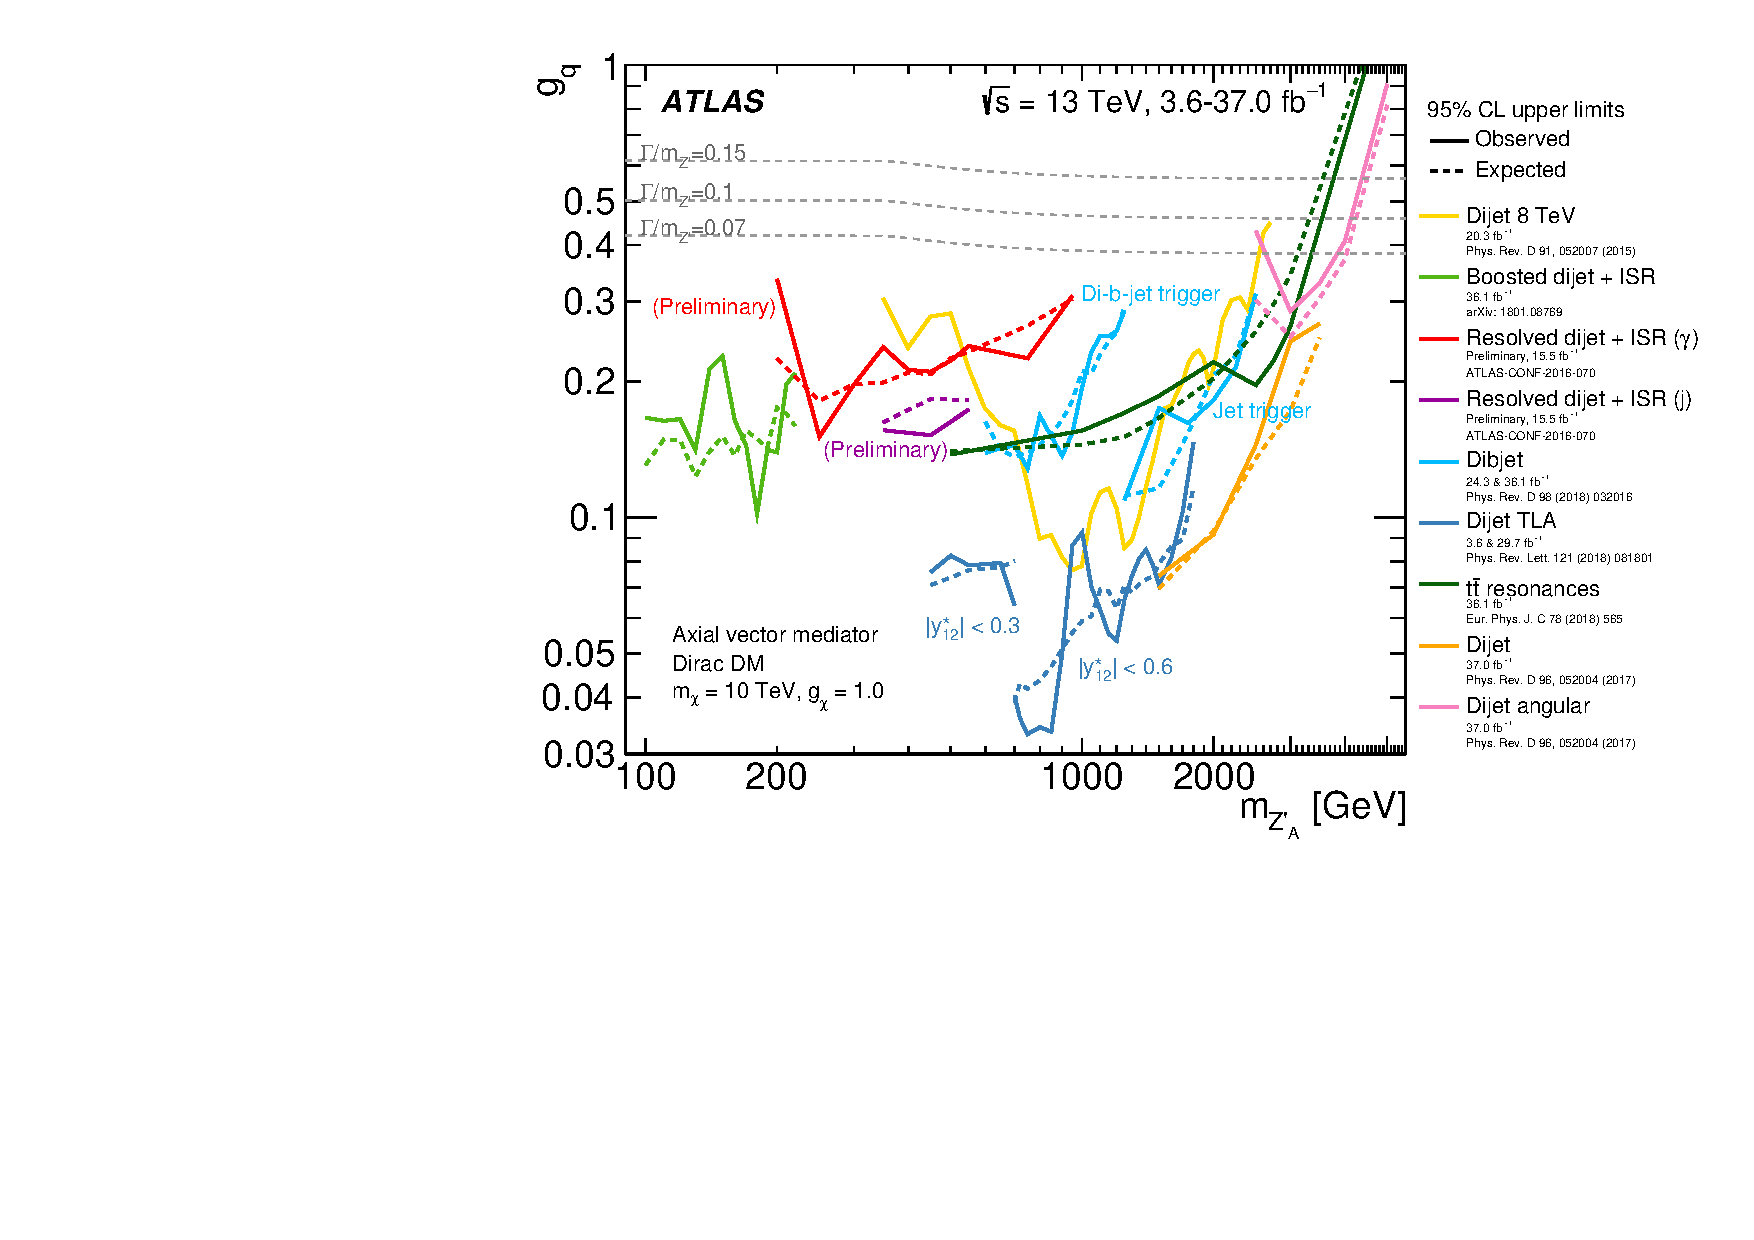
\includegraphics[width=\linewidth]{analysis/darkmatter_coupling_summary.pdf}
 \caption[Dijet search contours for $95\%$ CL upper limits on the coupling $g_{q}$ for the leptophobic axial-vector $\Zprime_{A}$ model.]{%
 Dijet search contours for $95\%$ CL upper limits on the coupling $g_{q}$ as a function of the resonance mass $m_{\Zprime_{A}}$ for the leptophobic axial-vector $\Zprime_{A}$ model.
 The expected limits from each search are indicated by dotted lines.
 The TLA dijet analysis has two parts, employing different datasets with different selections in the rapidity difference $y^{*}$ as indicated.
 The yellow contour shows the results of the dijet search using $20.3~\mathrm{fb}^{-1}$ of $8~\TeV$ data.
 Coupling values above the solid lines are excluded, as long as the signals are narrow enough to be detected using these searches.
 The TLA dijet search with $\abs{y^{*}} < 0.6$ is sensitive up to $\Gamma/m_{\Zprime} = 7\%$, the TLA dijet with $\abs{y^{*}} < 0.3$ and dijet + ISR searches are sensitive up to $\Gamma/m_{\Zprime} = 10\%$, and the dijet and dibjet searches are sensitive up to $\Gamma/m_{\Zprime} = 15\%$.
 The dijet angular analysis is sensitive up to $\Gamma/m_{\Zprime} = 50\%$.
 No limitation in sensitivity arises from large width resonances in the $t\bar{t}$ resonance analysis.
 Benchmark width lines are indicated in the canvas.
 The $\Gamma/m_{\Zprime} = 50\%$ lies beyond the canvas borders~\cite{EXOT-2017-32}.}
 \label{fig:darkmatter_coupling_summary}
\end{figure}

\begin{figure}[htbp]
 \centering
 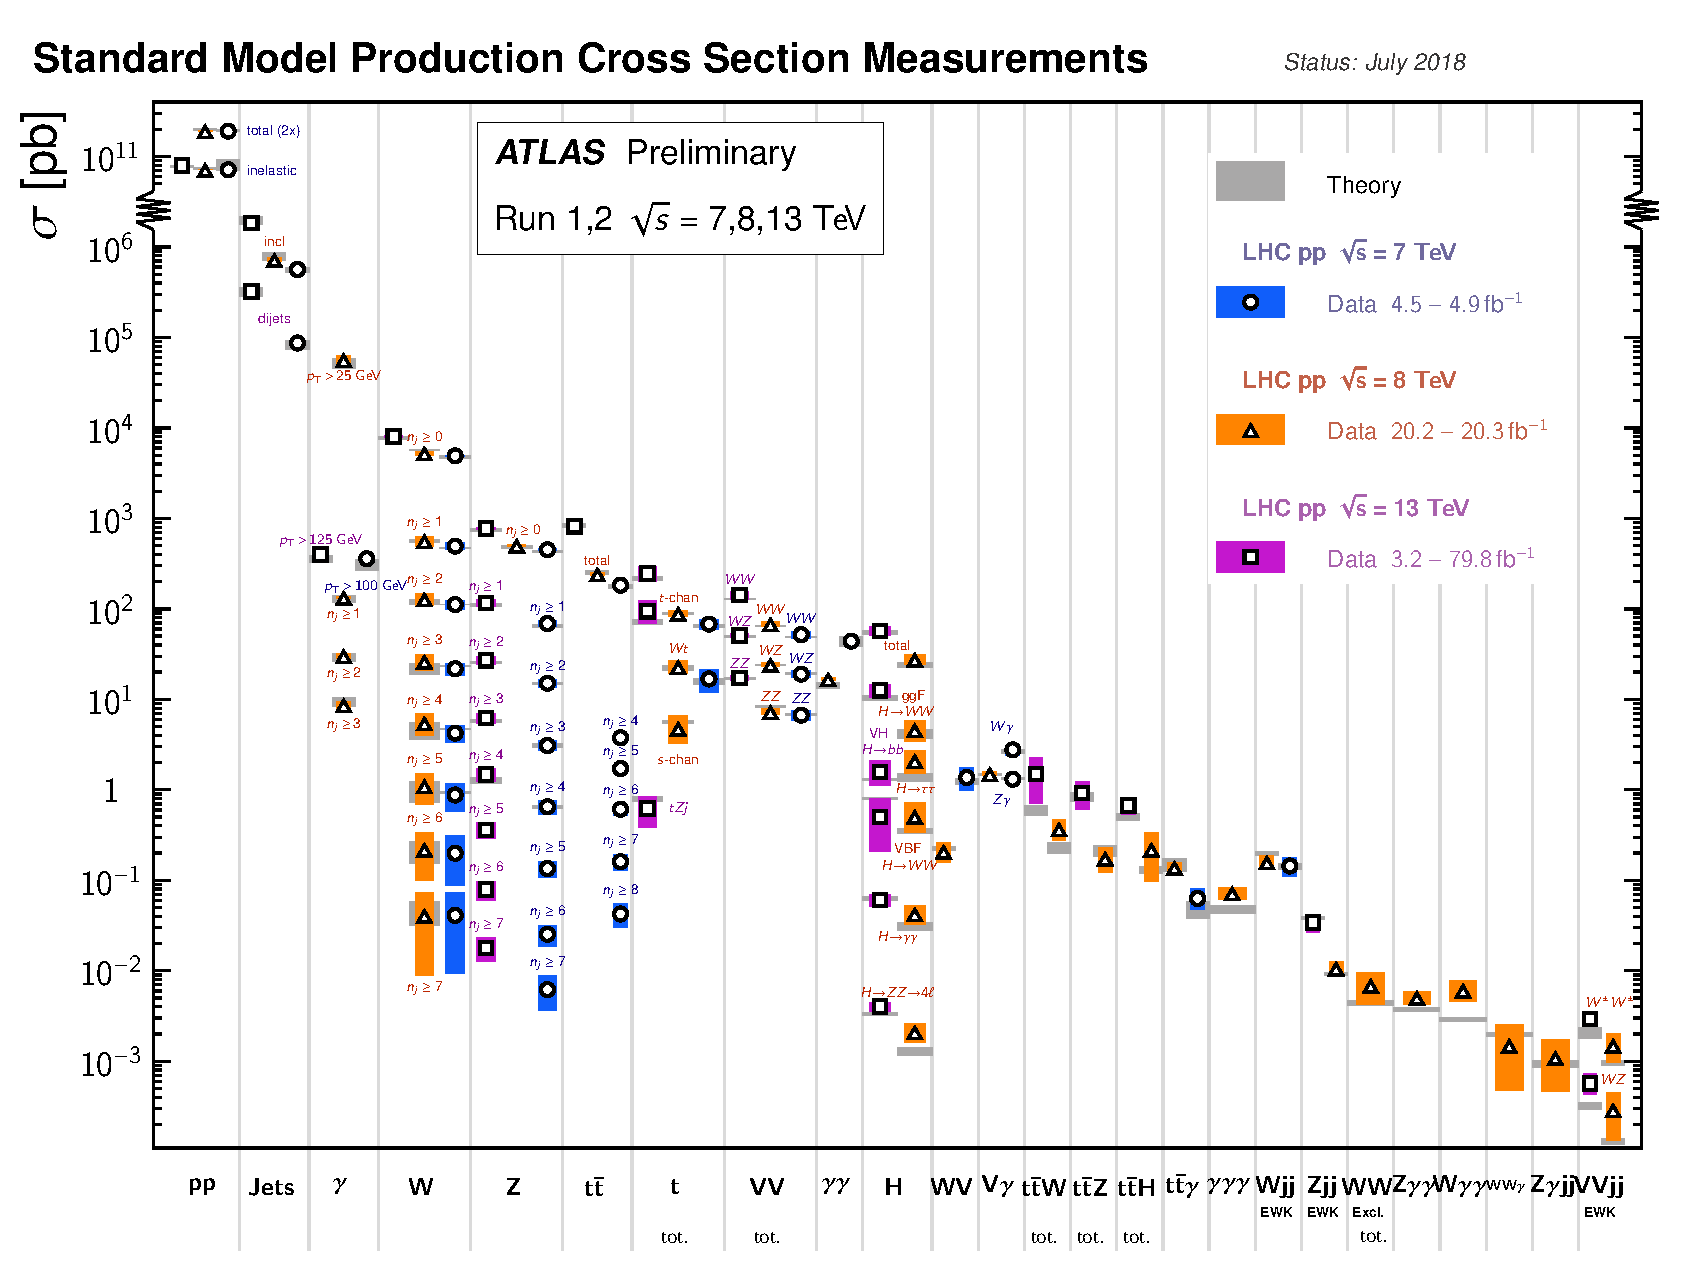
\includegraphics[width=\linewidth]{analysis/SM_fiducial_cross_section_summary.eps}
 \caption[Summary of several Standard Model total and fiducial production cross section measurements.]{%
  Summary of several Standard Model total and fiducial production cross section measurements, corrected for leptonic branching fractions, compared to the corresponding theoretical expectations.
  All theoretical expectations were calculated at NLO or higher.
  The luminosity used for each measurement is indicated close to the data point.
  Some measurements have been extrapolated using branching ratios as predicted by the Standard Model for the Higgs boson.
  Uncertainties for the theoretical predictions are quoted from the original ATLAS papers.
  They were not always evaluated using the same prescriptions for PDFs and scales.
  The $W\gamma$ and $Z\gamma$ theoretical cross sections have non-perturbative corrections applied to the NNLO fixed order calculations (PRD 87, 112003 (2013)).
  Not all measurements are statistically significant yet~\cite{web:ATLAS_SM_summary_plots}.}
 \label{fig:SM_fiducial_cross_section_summary}
\end{figure}

\begin{figure}[htbp]
 \centering
 \begin{subfigure}[t]{0.48\textwidth}
  \centering
  \includegraphics[width=\linewidth]{analysis/Hbb_ISR.pdf}
  \caption[Feynman diagram for the leading order production process at the LHC for ${\Hbb + \textrm{jet}}$.]{%
   Feynman diagram for the leading order production process at the LHC for ${\Hbb + \textrm{jet}}$ through gluon-gluon fusion.}
  \label{fig:signal_LO_diagram_Higgs}
 \end{subfigure}%
 \quad
 \begin{subfigure}[t]{0.48\textwidth}
  \centering
  \includegraphics[width=\linewidth]{analysis/Zprimebb_ISR.pdf}
  \caption[Feynman diagram for the leading order production process at the LHC for ${\Zprime + \textrm{jet}}$.]{%
   Feynman diagram for the leading order production process at the LHC for ${Z + \textrm{jet}}$ and ${\Zprime + \textrm{jet}}$ through quark annihilation.}
  \label{fig:signal_LO_diagram_Zprime}
 \end{subfigure}
 \caption[Feynman diagrams for the leading order production processes at the LHC for the signal events.]{%
  Feynman diagrams for the leading order production processes at the LHC of the Higgs and $\Zprime$ signal events.}
 \label{fig:signal_LO_diagrams}
\end{figure}

\begin{figure}[htbp]
 \centering
 \includegraphics[width=\linewidth]{analysis/Xbb_jet_recoil.pdf}
 \caption[Cartoon of a signal resonance recoiling of a high momentum jet.]{%
  Cartoon of a signal resonance, $X$, recoiling off a high momentum jet and decaying to a $b\bar{b}$ quark pair contained inside of a \largeR{} jet.}
 \label{fig:Xbb_jet_recoil}
\end{figure}

\begin{figure}[htbp]
 \centering
 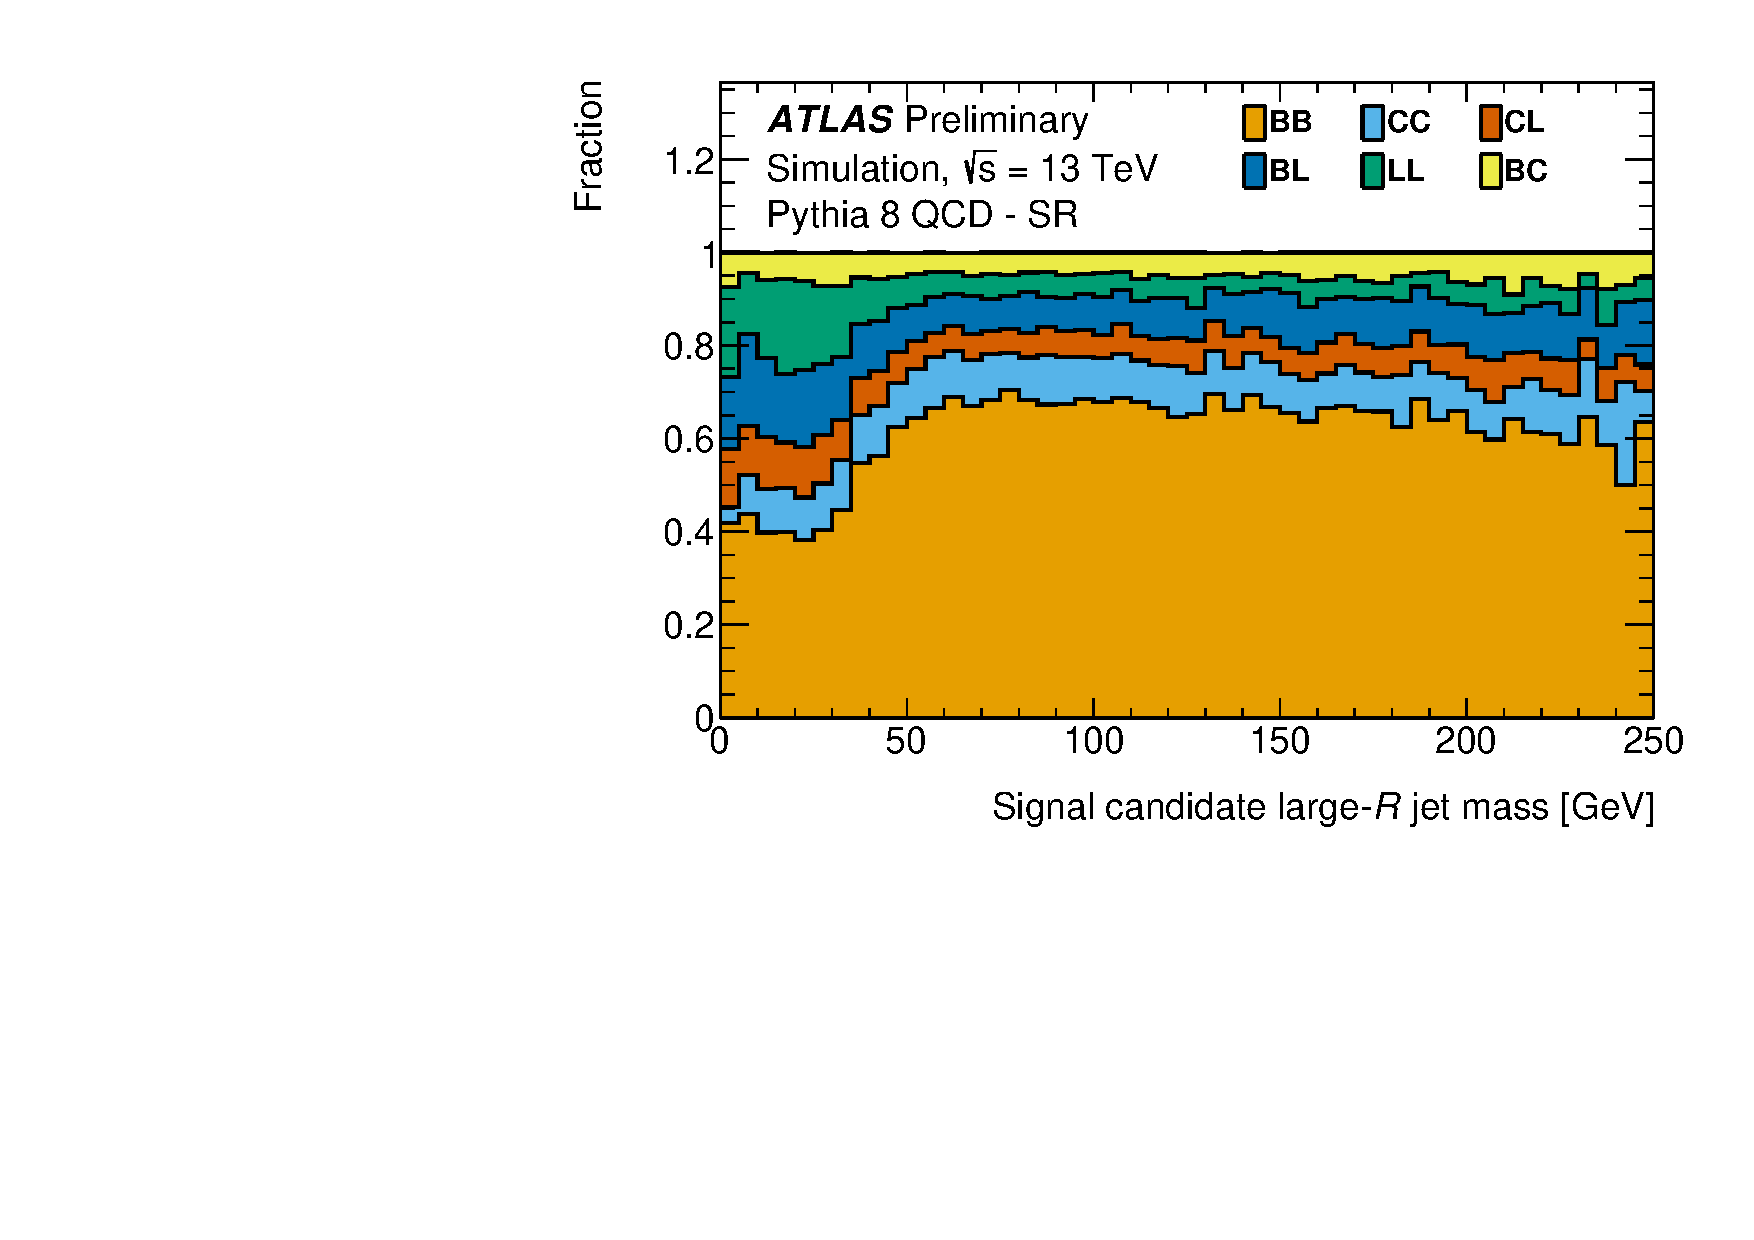
\includegraphics[width=0.6\linewidth]{analysis/TruthFlavourComposition_JetMass.pdf}
 \caption[Predicted flavor composition of the dijet background in the signal region.]{%
  Predicted flavor composition of the dijet background in the signal region based on the truth-matched hadron content of the two leading-$p_{T}$ track-jets associated to the signal candidate \largeR{} jet, with the B/C labels indicating the presence of a $b$/$c$-quark and L indicating the presence of a light quark or a gluon~\cite{ATLAS-CONF-2018-052}.}
 \label{fig:SR_flavor_composition}
\end{figure}

This chapter will cover the signal models and datasets in \Cref{sec:data_and_simulation}.
The $p_{T}$ requirements to have a fully efficient \largeR{} jet trigger across the 2015, 2016, and 2017 datasets is discussed in \Cref{sec:analysis_trigger}.
The construction of the signal region and supporting validation regions is covered in \Cref{sec:event_selection} and the effects of the resonant and non-resonant SM backgrounds in \Cref{sec:analysis_backgrounds}.
\Cref{sec:multijet_background_modeling} is devoted to my parametric modeling of the irreducible multijet background.
\Cref{sec:systematic_uncertainties} covers the effect of the leading systematic uncertainties on the analysis, and the results of the analysis are covered in \Cref{chapter:results}.

\clearpage
\section{Data and Simulation}\label{sec:data_and_simulation}

The analysis was done using $80.5~\ifb$ of data from ATLAS datasets collected in 2015, 2016, and 2017.
From the data quality monitoring, ATLAS produces XML files called ``Good Run Lists'' (GRLs) that are lists of all events in the data that have met the data quality criteria, ensuring high quality data for analysis.
The analysis uses three GRLs --- one for each year of data taking --- corresponding to annual luminosities of $3.2~\ifb$, $33.0~\ifb$, and $44.3~\ifb$.

\subsection{Simulated Signals}\label{sec:simulation_signal}

As both Higgs and $\Zprime$ are signals of the analysis two signal simulations were used: a SM Higgs boson decaying to $b\bar{b}$ and a leptophobic $\Zprime$ with democratic axial couplings to all quarks of mass less than $m_{\Zprime}/2$.
As the mass of the SM Higgs is known the analysis is optimized for the Higgs signal, while the production of $\Zprime$ simulation samples allows for searching a broad range of mass hypotheses.

The Higgs events were simulated with the three main production mechanisms at the LHC, seen in \Cref{fig:Higgs_production_diagrams}: gluon-gluon fusion, vector boson fusion, and Higgsstrahlung (associated $W$/$Z$ production).
These production modes respectively contribute to $50\%$, $30\%$, and $20\%$ of the total number of simulated signal events.
The ggF plus jet signal events are generated using the HJ+MiNLO~\cite{Hamilton:2015nsa} prescription with finite top quark mass using \textsc{Powheg-Box} 2~\cite{Campbell:2012am} and the NNPDF30 NNLO parton distribution function~\cite{Hamilton:2012rf} and then showered using \textsc{Pythia} 8.212~\cite{Sjostrand:2014zea} with the AZNLO tune and the CTEQ6L1~\cite{Pumplin:2002vw} parton distribution function.
The decay of the resulting $b$-hadrons is performed with EvtGen~\cite{Lange:2001uf}.
Similarly, with the exception of HJ+MiNLO, the VBF Higgs events are generated in the same manner.
Likewise, the Higgsstrahlung events are generated using \textsc{Pythia} 8.212 with the AZNLO tune and the CTEQ6L1 parton distribution function, with the decay of $b$-hadrons done with EvtGen.
As \textsc{Pythia} does not include $gg \to ZH$ the cross section is corrected to the LHC Higgs cross section working group recommendation~\cite{MelladoGarcia:2150771}.

The samples of $\Zprime$ decaying to two quarks and produced with an associated jet were generated using a simplified dark matter \textsc{MadGraph5_aMC@NLO} model~\cite{Abercrombie:2015wmb} and the NNPDF30 LO parton distribution function.
The events are showered using \textsc{Pythia 8} with the A14 tune and the NNPDF23 LO parton distribution function~\cite{Carrazza:2013axa} and the decay of $b$-hadrons is done with EvtGen.
To ensure a sufficiently large number of $\Zprime$ events at high $p_{T}$ all events are required to have an anti-$k_{T}$ $R = 0.6$ truth jet with $p_{T} > 350~\GeV$ before the detector simulation.
To enhance the truth jet filter efficiency \textsc{MadGraph5_aMC@NLO} is configured to save only simulated events that contain a patron with $p_{T} > 100~\GeV$.
Separate orthogonal samples for decays to light quarks $\left(\Zprime \to q\bar{q}\right)$ and $b$-quarks $\left(\Zprime \to b\bar{b}\right)$ are also produced to create datasets that are enhanced in $\Zprime \to b\bar{b}$ events.
As the search range of the analysis is between $100~\GeV$ and $200~\GeV$ signal samples are generated for the mass hypotheses of $m_{\Zprime} \in \left\{100, 125, 150, 175, 200, 250\right\}~\GeV$ to create events across the range of masses that might be used in studies or fits.
The simplified model defines an absolute axial coupling to SM quak-antiquark paris, $g_{q}$, that is assumed to be democratic.
The signal events are simulated with $g_{q} = 0.25$ corresponding to an approximate sensitivity estimate.
However, this choice does not have a significant effect on the kinematics of the reconstructed event as the natural width of the $\Zprime$ is smaller than the typical \largeR{} jet mass resolution in the $p_{T}$ and mass range of interest (i.e., about $10\%$ of the jet mass).
The total decay width of the $\Zprime$ is given as
\[
 \begin{split}
  \Gamma_{\Zprime} &= \Gamma_{SM} + \Gamma_{DM} \\
  &= \sum_{q \in \left(m_{q} < m_{\Zprime}/2\right)} \frac{3 m_{\Zprime} g_{q}^{2}}{12 \pi} \left(1 - \frac{\left(2m_{q}\right)^{2}}{m_{\Zprime}^{2}}\right)^{3/2} \\
  &\quad + \left\{\begin{array}{ll}
   \frac{3 m_{\Zprime} g_{DM}^{2}}{12 \pi} \left(1 - \frac{\left(2m_{DM}\right)^{2}}{m_{\Zprime}^{2}}\right)^{3/2}, & m_{DM} < m_{\Zprime}/2 \\
   0,                                                                                                               & \mathrm{otherwise},
  \end{array}\right.
 \end{split}
\]
though the presence of the dark matter particle, $\chi$, in the simplified model is integrated out by setting a very large mass of $m_{\chi} = 10~\TeV$ and then $g_{DM} = 1$, reducing the effective width in the simulation to
\[
 \Gamma_{\Zprime}\left(m_{\Zprime}, g_{q}\right) = \sum_{q \in \left(m_{q} < m_{\Zprime}/2\right)} \frac{3 m_{\Zprime} g_{q}^{2}}{12 \pi} \left(1 - \frac{\left(2m_{q}\right)^{2}}{m_{\Zprime}^{2}}\right)^{3/2}\,.
\]
As the cross section is proportional to $g_{q}^2$, the cross section at other values of $g_{q}$ can be determined from scaling the cross section used in the simulation,
\begin{equation}
 \sigma_{g_{q}'} = \sigma_{g_{q}} \left(\frac{g_{q}'}{g_{q}}\right)^{2}.
 \label{eq:g_q_scaling}
\end{equation}

\subsection{Simulated Backgrounds}\label{sec:simulation_background}

Simulation of the expected Standard Model backgrounds is used in the development of the non-resonant background processes and are used to model the resonant background processes.
Dijet events from QCD interactions are simulated using \textsc{Pythia 8.186} with the A14 tune and the NNPDF23 LO PDF and the decay of $b$-hadrons is done with EvtGen.
To achieve a constant statistical uncertainty over the large energy range weighted events are generated with a flat jet $p_{T}$ spectrum and split into multiple samples before reconstruction using an anti-$k_{t}$ $R=0.6$ jet algorithm run on the final-state truth particles.

The hadronically decaying $W$ and $Z$ events, with a maximum of four additional partons at leading order, were generated using \textsc{Sherpa} 2.1.1 with the CTO parton distribution function and were separated into multiple orthogonal samples based on the $p_{T}$ of the vector boson.
Leptonically decaying $W$ and $Z$ events are also produced with a maximum of two additional partons at leading order and a maximum of four at NLO.
These are used to correct the cross section of the hadronic sample by applying a multiplicative factor to scale the hadronic cross section to the leptonic sample cross section.
These ``$k$-factors'' are $1.28$ for the $W+\mathrm{jets}$ and $1.37$ for the $Z+\mathrm{jets}$~\cite{EXOT-2017-01}.
Alternate hadronic decay samples of $W+\mathrm{jets}$ and $Z+\mathrm{jets}$ were generated using \textsc{Herwig++} 2.7.1~\cite{Bahr:2008pv}.
However, unlike the \textsc{Sherpa} samples, only one additional parton is included in the matrix element.
The UEEE-4 underlying event tune~\cite{Buckley:2018wdv} was used with the CTEQ6L1 parton distribution function.

The simulated $\ttbar$ events were generated at tree-level using \textsc{Powheg-Box} 2 and the NNPDF30 NLO parton distribution function.
The hadronization of was performed using \textsc{Pythia} 8.230 with the A14 tune and the NNPDF23 parton distribution function and the decay of $b$-hadrons is performed using EvtGen.
The events are separated into categories based on whether both tops decayed hadronically, if only one of decayed hadronically, and if both tops decayed leptonically.
An additional set of $\ttbar$ events was generated using \textsc{Sherpa} 2.2.1 using the NNPDF30 parton distribution function, where independent samples were generated for the three decay categories.
This sample was used to cross-check the main $\ttbar$ samples generated with \textsc{Powheg-Box} 2 + \textsc{Pythia} 8.

\section{Large-$R$ Jet Trigger}\label{sec:analysis_trigger}

The trigger used in the analysis is a \largeR{} jet trigger.
However, as the amount of pile-up increased over the course of LHC Run 2, as seen in \Cref{fig:mu_2015_2017}, different \largeR{} trigger algorithms were used to maintain low offline thresholds for data recording.
This requires that a different trigger algorithm be used for the 2015, 2016, and 2017 data.
All triggers require the presence of a \largeR{} jet reconstructed in the \gls{HLT} with variations of ungroomed (a10) and \largeR{} jets trimmed (a10t) with the same settings as offline \largeR{} jets.
The 2015 trigger requires an ungroomed \largeR{} jet with $p_{T} > 360~\GeV$, while in 2016 the threshold is $420~\GeV$.
The 2017 trigger requires a trimmed online jet with a threshold of $460~\GeV$.
As shown in \Cref{table:annual_triggers}, the chosen triggers become fully efficient at different $p_{T}$ thresholds for offline \largeR{} jets.
As they are all fully efficient for $p_{T} > 480~\GeV$ and in an effort to simplify the analysis strategy a trimmed offline jet with $p_{T} > 480~\GeV$ is required for triggers across all years.

\begin{table}[htpb]
 \centering
 \caption[Summary of the triggers used in the analysis.]{%
  Summary of the \largeR{} jet triggers used in the analysis for the data taking periods of 2015, 2016, and 2017.}
 \begin{tabular}{@{}rlrr@{}}
  \toprule
  Year   & Trigger Name                 & Offline $p_{T}$ Threshold~$(\GeV)$ & Luminosity~$\left(\ifb\right)$ \\ \midrule
  $2015$ & HLT_j360_a10_lcw_sub_L1J100  & $410$                              & $3.2$                          \\
  $2016$ & HLT_j420_a10_lcw_L1J100      & $450$                              & $33.0$                         \\
  $2017$ & HLT_j460_a10t_lcw_jes_L1J100 & $480$                              & $44.3$                         \\
  \bottomrule
 \end{tabular}
 \label{table:annual_triggers}
\end{table}

\section{Signal Event Selection}\label{sec:event_selection}

All simulation and data are preprocessed to require events with at least two \largeR{} jets with $p_{T} > 200~\GeV$ before calibration.
Jets are further selected after calibration to be trimmed \largeR{} jets with $p_{T} > 250~\GeV$ and $\abs{\eta} < 2$.
Events are further preselected by requiring the leading $p_{T}$ \largeR{} jet to satisfy $p_{T} > 480~\GeV$ and the sub-leading $p_{T}$ \largeR{} jet to have $p_{T} > 250~\GeV$, which ensures that all events meet the trigger requirements.
To select the signal jet candidate --- the \largeR{} jet assumed to contain the decay products of the $\Zprime$ or the Higgs boson --- the following criteria must be met.
The \largeR{} jet must be sufficiently boosted with $p_{T} > 2m_{J}$, and it must contain at least two variable radius track-jets each with $p_{T} > 10~\GeV$.
To help prevent contamination of gluon splitting to heavy flavor quarks, an additional requirement is made that the distance between the two leading $p_{T}$ VR track-jet axes is greater than the radius of the smaller of the two VR track-jet (the leading $p_{T}$ VR track-jet), $\Delta R_{VR}/\mathrm{min\,} R_{VR} > 1$.
The highest $p_{T}$ \largeR{} jet that passes all of these requirements is then taken to be the signal candidate, and the next highest $p_{T}$ \largeR{} jet is taken to be the associated jet.
Additionally, any events with muons with $p_{T} > 40~\GeV$ opposite the signal candidate, $\Delta \phi > 2\pi/3$, are removed to ensure that the signal candidate events are orthogonal to a $\ttbar$ control region that will be constructed from these muon events.
The signal candidate selection process is summarized visually in \Cref{fig:event_selection}.

\begin{figure}[htbp]
 \centering
 \includegraphics[width=0.9\linewidth]{analysis/event_selection.pdf}
 \caption[Diagram of the signal candidate event selection process.]{%
  Diagram of the signal candidate event selection process.}
 \label{fig:event_selection}
\end{figure}

Once the signal candidate jet is chosen, events are further classified based on how many of the leading $p_{T}$ VR track-jets in the signal candidate \largeR{} jet pass $b$-tagging criteria.
A ``loose'' $b$-tagging working point is established at $85\%$ $b$-tagging efficiency, and a ``tight'' $b$-tagging working point is established at $77\%$ $b$-tagging efficiency.%
\footnote{The $b$-tagging efficiencies are determined through applying the $b$-tagging algorithm to offline-reconstructed jets from an unbiased sample of Monte Carlo simulated $t\bar{t}$ events, where jets are labeled according to their hadron content.}
The $77\%$ efficiency working point is selected to optimize signal significance.
Signal candidate events with zero loose $b$-tagged track-jets define a control region for non-resonant background estimation studies (\CRQCD).
Events with exactly two tight $b$-tagged track-jets form the signal region (SR).

The efficiencies and yields of the resonant backgrounds and the signal processes under the event selection criteria in the $0$-tag control region and the signal region are given in \Cref{table:efficiencies_and_yields}, where the efficiency is defined as the fraction of events that pass the leading \largeR{} jet $p_{T} > 480~\GeV$ event selection requirement that get classified in the particular region.
The composition of the vector boson, $\ttbar$, and $\Hbb$ resonant components in the $0$-tag control region and signal region are shown in \Cref{table:fractional_composition}.
As expected, in the \CRQCD{} the $W+\mathrm{jets}$ contribution is dominant for the vector boson component and in the signal region is primarily from $Z+\mathrm{jets}$.
The $\ttbar$ contribution is roughly equivalent in both the \CRQCD{} and the SR with approximately $60\%$ resulting from hadronic decays.
In both regions the dominant component of $\Hbb$ is from gluon-gluon fusion production. In the signal region gluon-gluon fusion contributes $53\%$, followed by VBF production at $25\%$, and Higgsstrahlung at $22\%$.

\begin{table}[htpb]
 \centering
 \caption[Efficiencies and yields of resonant backgrounds and the signal processes.]{%
  The efficiencies and yields in the $0$-tag control region (\CRQCD{}) and signal region (SR) for the non-QCD background, the Higgs boson, and $\Zprime$ signals and data.
  The yields in the \CRQCD{} are given for the luminosity used for the background estimate of the non-resonant dijet process.
  The efficiencies are relative to the leading \largeR{} jet $p_{T} > 480~\GeV$ requirement.}
 \begin{adjustbox}{max width=\textwidth}
  \begin{tabular}{@{}lrrrrr@{}}
   \toprule
   Process                             & \CRQCD{} Eff. $(\%)$ & \CRQCD{} Yield in $1.4~\ifb$ & SR Eff. $(\%)$ & SR Yield in $80.5~\ifb$ \\ \midrule
   $W \to q\bar{q} + \mathrm{jets}$    & $51.3$               & $3810$                       & $0.4$          & $1500$                  \\
   $Z \to q\bar{q} + \mathrm{jets}$    & $46.2$               & $1470$                       & $3.4$          & $6200$                  \\
   $t\bar{t}$                          & $25.9$               & $1929$                       & $2.5$          & $10550$                 \\
   $\Hbb$                              & $24.3$               & $5$                          & $17.9$         & $216$                   \\
   \phantom{$\Hbb$\quad}~ggF           & $23.6$               & $2$                          & $19.4$         & $115$                   \\
   \phantom{$\Hbb$\quad}~VBF           & $15.8$               & $1$                          & $20.7$         & $53$                    \\
   \phantom{$\Hbb$\quad}~$WH$          & $32.4$               & $1$                          & $12.0$         & $26$                    \\
   \phantom{$\Hbb$\quad}~$ZH$          & $30.5$               & $1$                          & $15.8$         & $21$                    \\
   $\Zprime$ $\left(m=100~\GeV\right)$ & $43.9$               & $1530$                       & $4.1$          & $8200$                  \\
   $\Zprime$ $\left(m=125~\GeV\right)$ & $43.6$               & $1440$                       & $3.8$          & $7300$                  \\
   $\Zprime$ $\left(m=150~\GeV\right)$ & $43.5$               & $1360$                       & $3.7$          & $6700$                  \\
   $\Zprime$ $\left(m=175~\GeV\right)$ & $42.8$               & $1240$                       & $3.3$          & $5550$                  \\
   $\Zprime$ $\left(m=200~\GeV\right)$ & $41.8$               & $1127$                       & $3.2$          & $4910$                  \\
   Data                                & $38.7$               & $519710$                     & $0.6$          & $484600$                \\
   \bottomrule
  \end{tabular}
 \end{adjustbox}
 \label{table:efficiencies_and_yields}
\end{table}

\begin{table}[htpb]
 \centering
 \caption[The fractional composition of the different resonant contributions in the $0$-tag control region and signal region.]{%
  The fractional composition of the different resonant contributions in the $0$-tag control region (\CRQCD{}) and the signal region (SR).}
 \begin{tabular}{@{}lrr@{}}
  \toprule
  Process                                   & \CRQCD{} Fraction & SR Fraction \\ \midrule
  $\Vjets$                                  &                   &             \\
  \phantom{$\Vjets$\quad} $Z+\mathrm{jets}$ & $0.28$            & $0.80$      \\
  \phantom{$\Vjets$\quad} $W+\mathrm{jets}$ & $0.72$            & $0.20$      \\
  $t\bar{t}$                                &                   &             \\
  \phantom{$t\bar{t}$\quad} Hadronic        & $0.58$            & $0.63$      \\
  \phantom{$t\bar{t}$\quad} Semi-leptonic   & $0.38$            & $0.34$      \\
  \phantom{$t\bar{t}$\quad} Dileptonic      & $0.04$            & $0.03$      \\
  $\Hbb$                                    &                   &             \\
  \phantom{$\Hbb$\quad} ggF                 & $0.49$            & $0.53$      \\
  \phantom{$\Hbb$\quad} VBF                 & $0.17$            & $0.25$      \\
  \phantom{$\Hbb$\quad} $WH$                & $0.21$            & $0.12$      \\
  \phantom{$\Hbb$\quad} $ZH$                & $0.12$            & $0.10$      \\
  \bottomrule
 \end{tabular}
 \label{table:fractional_composition}
\end{table}

\section{Backgrounds}\label{sec:analysis_backgrounds}

\subsection{$\Vjets$}

As this analysis is looking for resonances on the tails of the $\Vjets$ and $\ttbar$ mass distributions it is important to ensure that the Monte Carlo based templates don't have statistical fluctuations that could hide possible signals.
To avoid this, parametric shapes are fitted to the MC-based templates ensuring that the tails are well modeled without fluctuations.
For the $\Vjets$ and signal templates the sum of three Gaussians plus a constant term are fitted to the templates, and for the $\ttbar$ a double-sided Crystal Ball~\cite{Gaiser:1982yw} is used.
All systematic variation histograms are also fitted with the same functional choices.

\subsection{$\ttbar$}\label{sec:ttbar}

As seen in \Cref{table:efficiencies_and_yields}, boosted $\ttbar$ events are a significant background in the signal region.
However, current generation MC generators are not able to predict the $\ttbar$ cross section well in the boosted regime~\cite{ATL-PHYS-PUB-2018-009}.
To correct the $\ttbar$ yield accordingly in the SR a $k$-factor is applied to the normalization.
This $k$-factor is obtained from fitting the normalization of the $\ttbar$ MC template to a $\ttbar$ enriched control region of the data (\CRttbar{}).
The resulting $k$-factor is applied to the $\ttbar$ MC template normalization in the signal region, with the $k$-factor's uncertainty used as a Gaussian prior on the normalization.

The $\ttbar$ enriched control region uses the same selections for the signal candidate \largeR{} jet in terms of the corresponding $p_{T}$ cuts.
Three regions are defined by requiring zero, one, or two $b$-tags in the two leading $p_{T}$ track-jets of the signal candidate, though the region with one $b$-tagged track-jet is taken as the \CRttbar{}, given that it exploits the single $b$-quark in a top quark decay.
The other regions are used to validate the extrapolation of the $k$-factor into the \CRQCD{} and SR topologies.
The sample further requires the muon from the semi-leptonic decay of the second top quark to be in the opposite hemisphere of the signal jet.
This is implemented by applying a cut of $\Delta \phi \left(\mathrm{muon}, \mathrm{signal~jet}\right) > 2\pi/3$, which significantly reduces the QCD and $\Vjets$ contribution to the signal region which reducing the $\ttbar$ contribution by roughly a factor of three.%
\footnote{This is to be expected as the leptonic decay modes of the $W$ have roughly uniform branching fractions, $BR\left(W \to \mu\, \nu_{\mu}\right)/BR\left(W \to \ell \,\nu_{\ell}\right) \simeq 1/3$.}
To further reduce contamination from multijet events, a cut of $p_{T} > 40~\GeV$ is applied to muon to veto softer muons resulting from multijet events.
Finally, at least one tight $b$-tagged track-jet is required to be within $\Delta R \left(\mathrm{jet}, \mathrm{muon}\right) < 1.5$ to reduce contamination from $V\left(\to \ell\ell\,\right)+\mathrm{jets}$ and $VV$ events.
The \CRttbar{} selection criteria are summarized visually in \Cref{fig:ttbar_CR_selection}.

\begin{figure}[htbp]
 \centering
 \includegraphics[width=\linewidth]{analysis/ttbar_CR.pdf}
 \caption[Diagram of the $t\bar{t}$ control region selection criteria.]{%
  Diagram of the \CRttbar{} selection criteria.}
 \label{fig:ttbar_CR_selection}
\end{figure}

The $\ttbar$ MC template is fit to the data in the \CRttbar{} over the mass range of $70~\GeV$ to $230~\GeV$ and the uncertainty on the fit is determined from running the Bayesian Analysis Toolkit with \largeR{} jet energy scale and jet energy resolution variations as nuisance parameters, which will be described in \Cref{sec:systematic_uncertainties}.
This results in a $k$-factor of $0.84 \pm 0.11$, which is then used to constrain the $t\bar{t}$ contribution in the final fit to the signal region data.


\section{Modeling of the Multijet Background}\label{sec:multijet_background_modeling}

The dominant background contribution in the SR is the non-resonant multijet process.
Its estimate through MC is not reliable due to the statistical precision and the underlying accuracy of the event generation.
A data-driven estimate is therefore employed by fitting the signal candidate \largeR{} jet mass distribution, $m_{J}$, in the SR with a parametric function and by validating the procedure using the data in the \CRQCD{}.
This data-driven approach is further motivated by the fact that the shape of the \CRQCD{} and the SR is very similar over the mass range of the fit, $70~\GeV$ to $230~\GeV$, as seen in \Cref{fig:fit_range_QCD_shape}.
The fit range extends beyond the $100~\GeV$ to $200~\GeV$ mass search range to provide additional points to help stabilize the fit.
As approximately $1.2~\ifb$ of data in the \CRQCD{} gives a similar yield as is expected from the full $80.5~\ifb$ dataset in the SR, I performed the fitting study in approximately 60 slices of $1.2~\ifb$ \CRQCD{} data.

\begin{figure}[htbp]
 \centering
 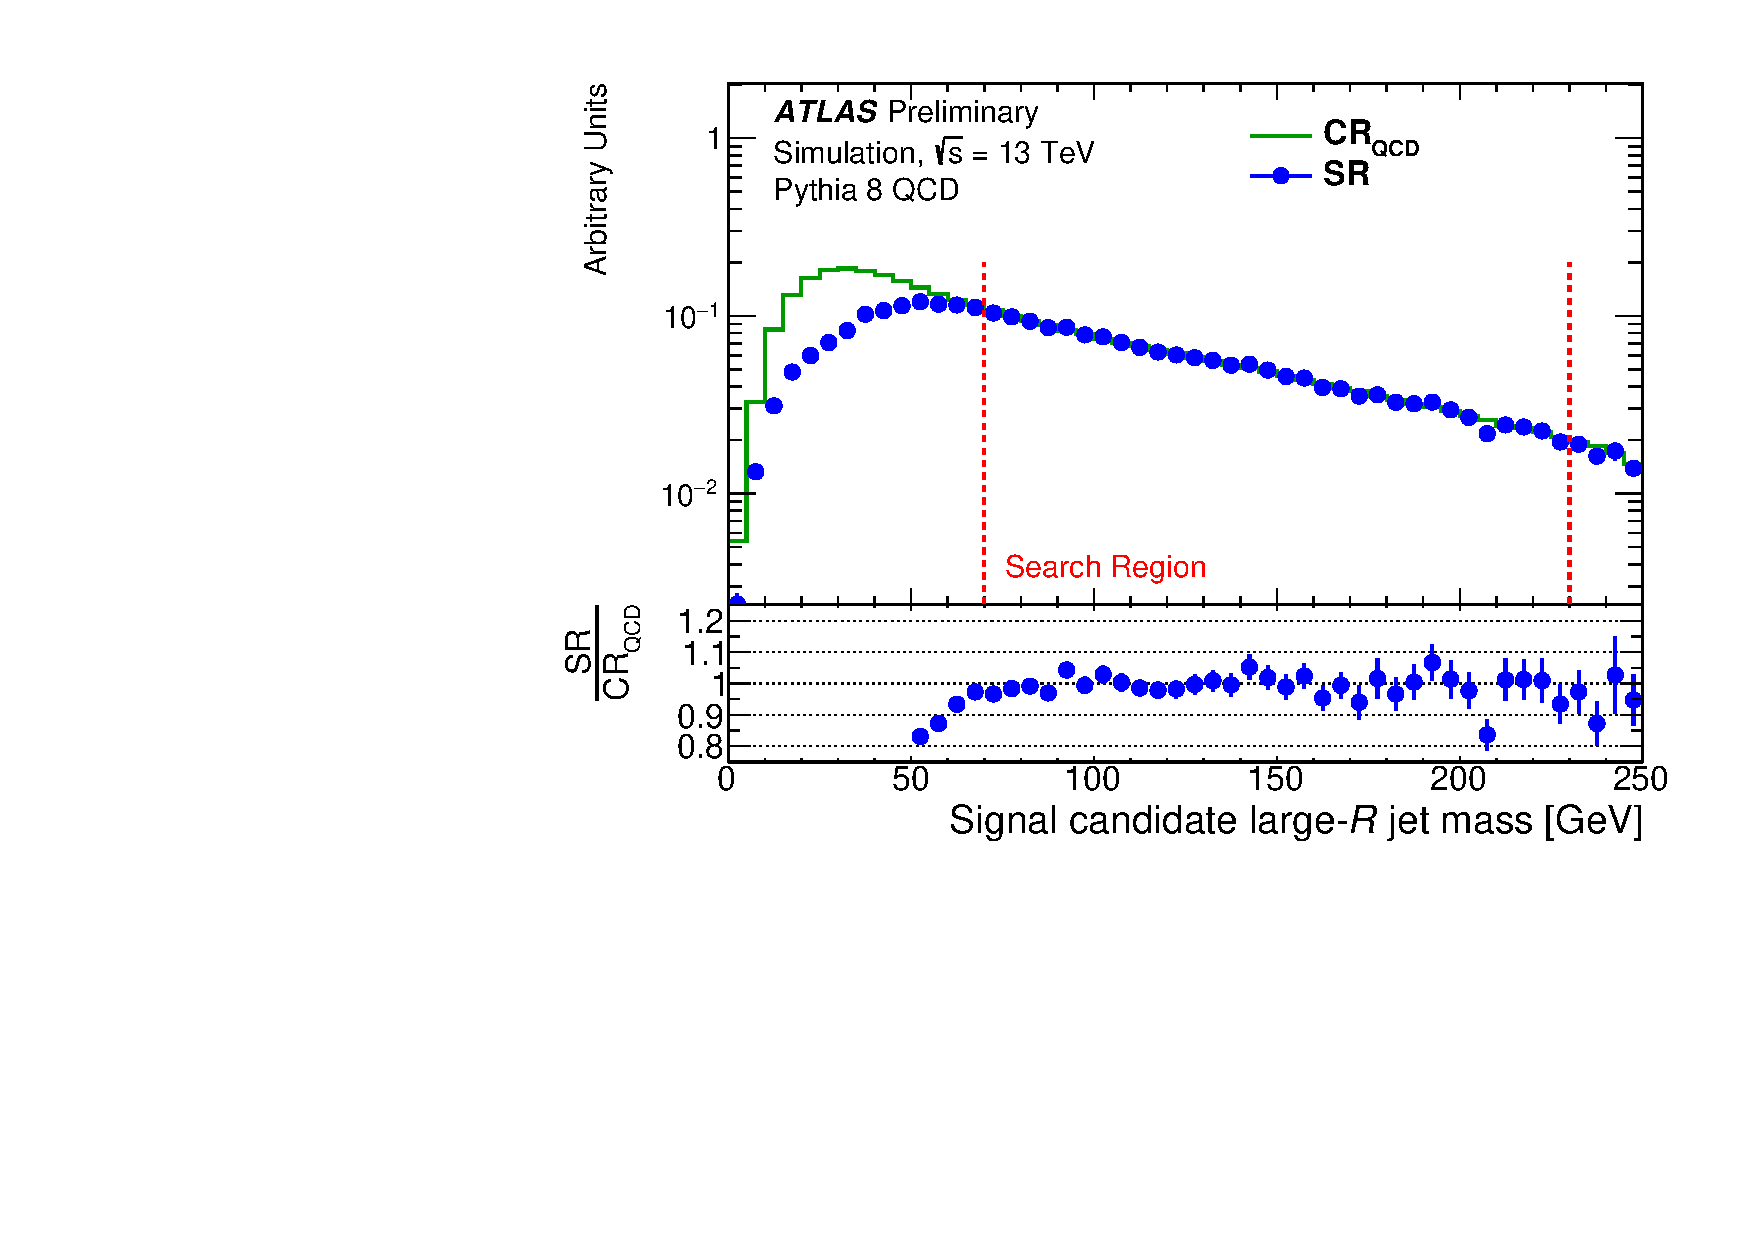
\includegraphics[width=\linewidth]{analysis/fit_range_QCD_shape.pdf}
 \caption[Comparison of the multijet background shape in the signal region and $0$-tag control region (\CRQCD{}).]{%
  The expected shape of the multijet background in the signal region and the \CRQCD{} normalized to the same event count between $70~\GeV < m_{J} < 230~\GeV$.}
 \label{fig:fit_range_QCD_shape}
\end{figure}

\subsection{Models Tested}\label{sec:models_tested}

To find a parametric function that fits the multijet background well, I investigated a selection of families of functions.
I considered multiple models, many of which proved intractable in fitting, but two families of models performed well across the \CRQCD{} data slices.
The functional forms of the families are the ``polynomial exponential'' --- taken to be the nominal model for the studies ---
\begin{equation}
 f_{n} \left(x \middle|\,\vec{\theta}\right) = \theta_{0}\, \exp\left(\sum_{i=1}^{n} \theta_{i}\,x^{i}\right), \quad x = \frac{m_{J} - 150~\GeV}{80~\GeV},
 \label{eq:poly_exp}
\end{equation}
and the alternative model, the Formal Laurent series,
\begin{equation}
 f_{n} \left(x \middle|\,\vec{\theta}\right) = a \sum_{i=0}^{n} \frac{\theta_{i}}{x^{i+1}}, \quad a=10^{5},\,x = \frac{m_{J} + 90~\GeV}{160~\GeV},
 \label{eq:formal_laurent}
\end{equation}
The parameterization of the polynomial exponential function maps the independent variable to $x \in \left[-1,1\right]$ for the fit range of $[70,230]~\GeV$, and the parameterization of the Formal Laurent series maps the independent variable to $x \in \left[1,2\right]$ over the same range.
This reparameterization is done, as I observed that it improved the numerical stability of the fit.
The scaling factor, $a$, for the Formal Laurent is not a free parameter; it is empirically chosen to keep the scale of the parameters at $\mathcal{O}(1)$.
The Formal Laurent series serves as a cross check for the polynomial exponential function models.
To focus only on the QCD part of the spectrum, the MC templates for the $W+\mathrm{jets}$, $Z+\mathrm{jets}$, and $\ttbar$ (scaled by their cross section times the luminosity of each slice and any relevant $k$-factors) are subtracted from the data.
This is done to decouple the study from any possible bias introduced by the fitting procedure.

\subsubsection{Likelihood ratio test}

Using Wilk's theorem, as described in \Cref{subsection:wilks_theorem}, the \pvalue{} for a likelihood ratio test statistic,
\[
 t_{\vec{\theta}} = -2 \ln \frac{\displaystyle L\left(\vec{\theta}_{a}\right)}{\displaystyle L\left(\vec{\theta}_{b}\right)},
\]
for models $f\left(x\,\middle|\,\vec{\theta}_{a}\right)$ and $f\left(x\,\middle|\,\vec{\theta}_{b}\right)$ can be computed efficiently.
If the \pvalue{} is below a given threshold, $\alpha$, the difference in the fits of the two models is considered statistically significant and the model with a greater number of parameters is favored.
Likewise, if the \pvalue{} is above the threshold, the difference is considered not to be statistically significant and the model with fewer number of parameters is favored.
The comparison is done for iteratively higher numbers of parameters until the result of the test shows that an additional parameter no longer significantly improves the fit.
The choice of threshold is in general arbitrary and specific to the circumstances of the fit being performed.
In the particular circumstances of the studies performed the changes in the \pvalue{} are quite abrupt, so it is reasonable to require a \pvalue{} threshold of $\alpha=0.1$.

\subsubsection{$F$-test}

The $F$-test~\cite{snecdecor1991statistical} is another statistical test that can be used to determine the minimum number of model parameters to describe the shape of a distribution from the $\chi^2$ of the model's fit.
The $F$-test statistic can be defined as
\begin{equation}
 F = \frac{\chi^2_1/\nu_1}{\chi^2_0/\nu_0},
\end{equation}
where $\chi^2_0$ is the smaller $\chi^2$ of the two fitted models being compared, and $\nu_{i}$ are the degrees of freedom for each fit.
The $F$-test statistic is distributed according to the $F$-distribution, and so the one-sided (one-tailed) \pvalue{} of this test statistic is then the value of the complementary cumulative distribution function of the $F$-distribution evaluated at the observed $F$,
\begin{equation}
 p\text{-value}\left(F_{\text{obs}}\right) = \textrm{CCDF}\left(x=F_{\text{obs}}\right) = 1 - I\left(\frac{\nu_{1} F_{\text{obs}}}{\nu_{0} + \nu_{1} F_{\text{obs}}}; \frac{\nu_{1}}{2}, \frac{\nu_{0}}{2}\right)
\end{equation}
where $I$ is the regularized incomplete beta function.

\subsection{Model Selection}\label{sec:model_selection}

For models of the same family that exhibited good reduced $\chi^2$ values during fitting, the likelihood ratio test and $F$-test were performed to select the favored model.
\Cref{fig:likelihood_ratio_test_polyexp} shows the results of the two statistical test being applied to the polynomial exponential family of functions, demonstrating that the 5 parameter model is favored as the minimum number of parameters to model the background distribution well.
\Cref{table:stat_test_parameters} summarizes the results of the statistical tests.

To check this result, I repeated the two statistical tests for the polynomial exponential family of functions for all \CRQCD{} data slices.
The relative frequencies of the observed \pvalue{}s for the tests are iteratively summed, as seen in \Cref{fig:empirical_CDF_polyexp}, producing an empirical cumulative distribution function (CDF) for the test \pvalue{}s.
It is seen that for the \emph{a priori} threshold of $\alpha=0.1$ that in a large majority of the cases the likelihood ratio test favors a 5 parameter model ($\textrm{CDF}_{4\textrm{v.}5}\left(0.1\right) > 0.9$) while in most cases the $F$-test favors a 4 parameter model ($\textrm{CDF}_{4\textrm{v.}5}\left(0.1\right) < 0.2$).
Given this contention and the very strong favoring of the 5 parameter model in the likelihood ratio test, the 5 parameter model is conservatively chosen to model the shape of the QCD background distribution.
\Cref{fig:5param_QCD_model_fit} shows the result of the fit in the original data slice with the selected 5 parameter QCD model.

\begin{table}[htbp]
 \centering
 \caption[The observed \pvalue{} for the likelihood ratio test and $F$-test for comparing the polynomial exponential model with different number of parameters.]{%
  The observed \pvalue{} for the likelihood ratio test and $F$-test for comparing the polynomial exponential model with different number of parameters.}
 \label{table:stat_test_parameters}
 \begin{tabular}{@{}crr@{}} \toprule
  Parameters in compared models & likelihood ratio test \pvalue{} & $F$-test \pvalue{} \\ \midrule
  4 v. 5                        & $0.0001$                        & $0.0748$           \\
  5 v. 6                        & $0.3355$                        & $0.4867$           \\
  \bottomrule
 \end{tabular}
\end{table}

\begin{figure}[htbp]
 \centering
 \begin{subfigure}[t]{0.48\textwidth}
  \centering
  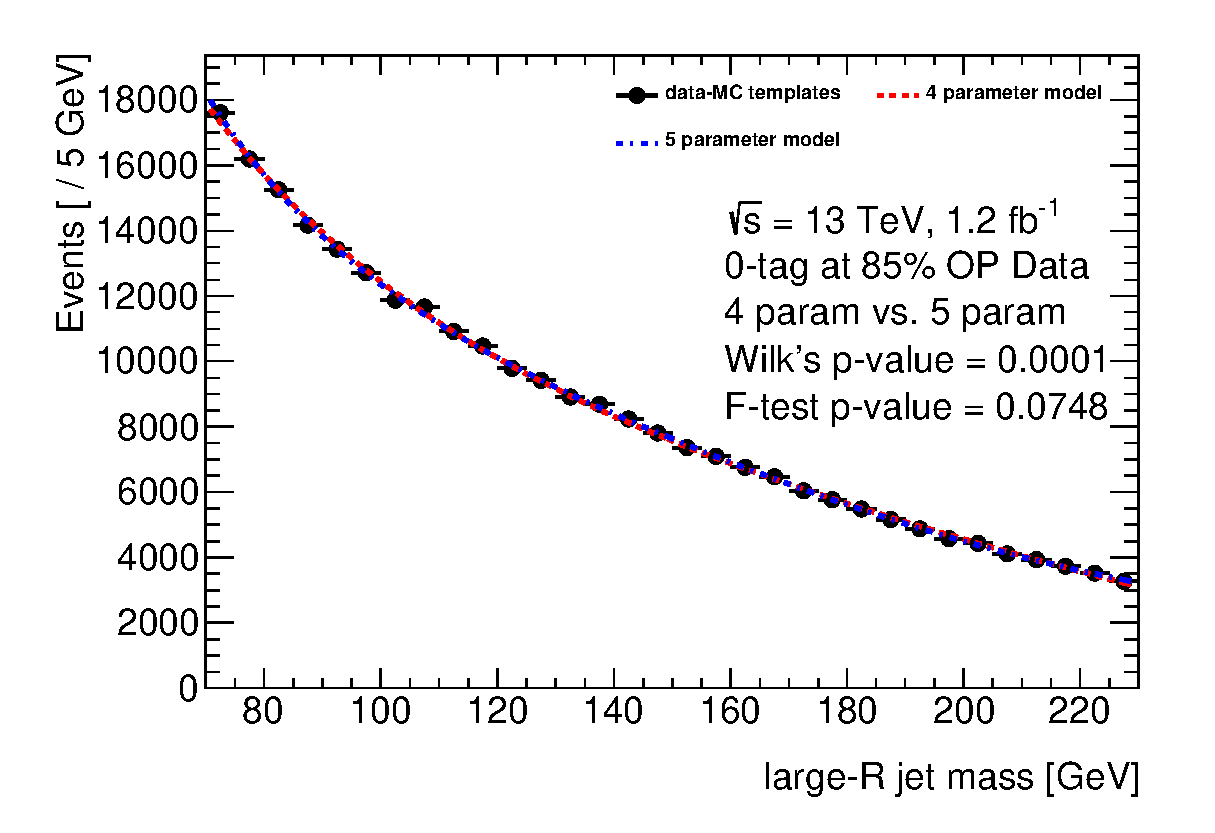
\includegraphics[width=\textwidth]{analysis/stat_test_exp_4_v_5params_CR_data.eps}
  \caption[Comparison of the 4 and 5 parameter polynomial exponential fit models.]{%
   Comparison of the 4 and 5 parameter polynomial exponential fit models to \CRQCD{} data minus resonant Monte Carlo templates.}
  \label{fig:stat_test_exp_4_v_5params}
 \end{subfigure}%
 \quad
 \begin{subfigure}[t]{0.48\textwidth}
  \centering
  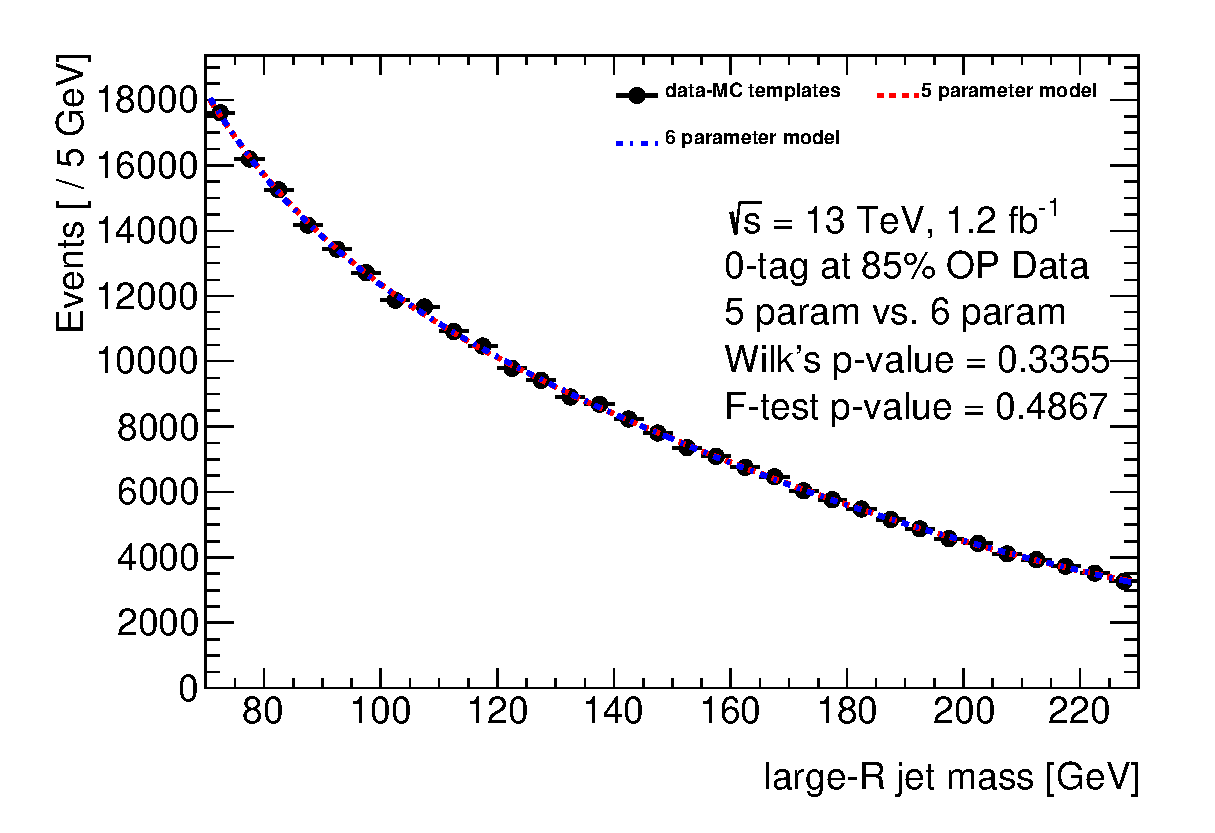
\includegraphics[width=\textwidth]{analysis/stat_test_exp_5_v_6params_CR_data.eps}
  \caption[Comparison of the 5 and 6 parameter polynomial exponential fit models.]{%
   Comparison of the 5 and 6 parameter polynomial exponential fit models to \CRQCD{} data minus resonant Monte Carlo templates.}
  \label{fig:stat_test_exp_5_v_6params}
 \end{subfigure}
 \caption[Results of the likelihood ratio test and $F$-test of comparing the polynomial exponential fit models.]{%
  The results of the likelihood ratio test and $F$-test of comparing the polynomial exponential fit models to \CRQCD{} data minus resonant Monte Carlo templates.
  Given the \pvalue{}s of the likelihood ratio test and $F$-test are $p < \left(\alpha=0.1\right)$ in the comparison between the 4 and 5 parameter models the 5 parameter model is selected as giving a statistically significant improvement to the fit.
  Given the large \pvalue{}s observed between the 5 and 6 parameter model, $p > 0.1$, the addition of a 6th parameter to the model does not contribute to a significant improvement in the fit.
  As a result, the 5 parameter model is favored.}
 \label{fig:likelihood_ratio_test_polyexp}
\end{figure}

\begin{figure}[htbp]
 \centering
 \begin{subfigure}[t]{0.48\textwidth}
  \centering
  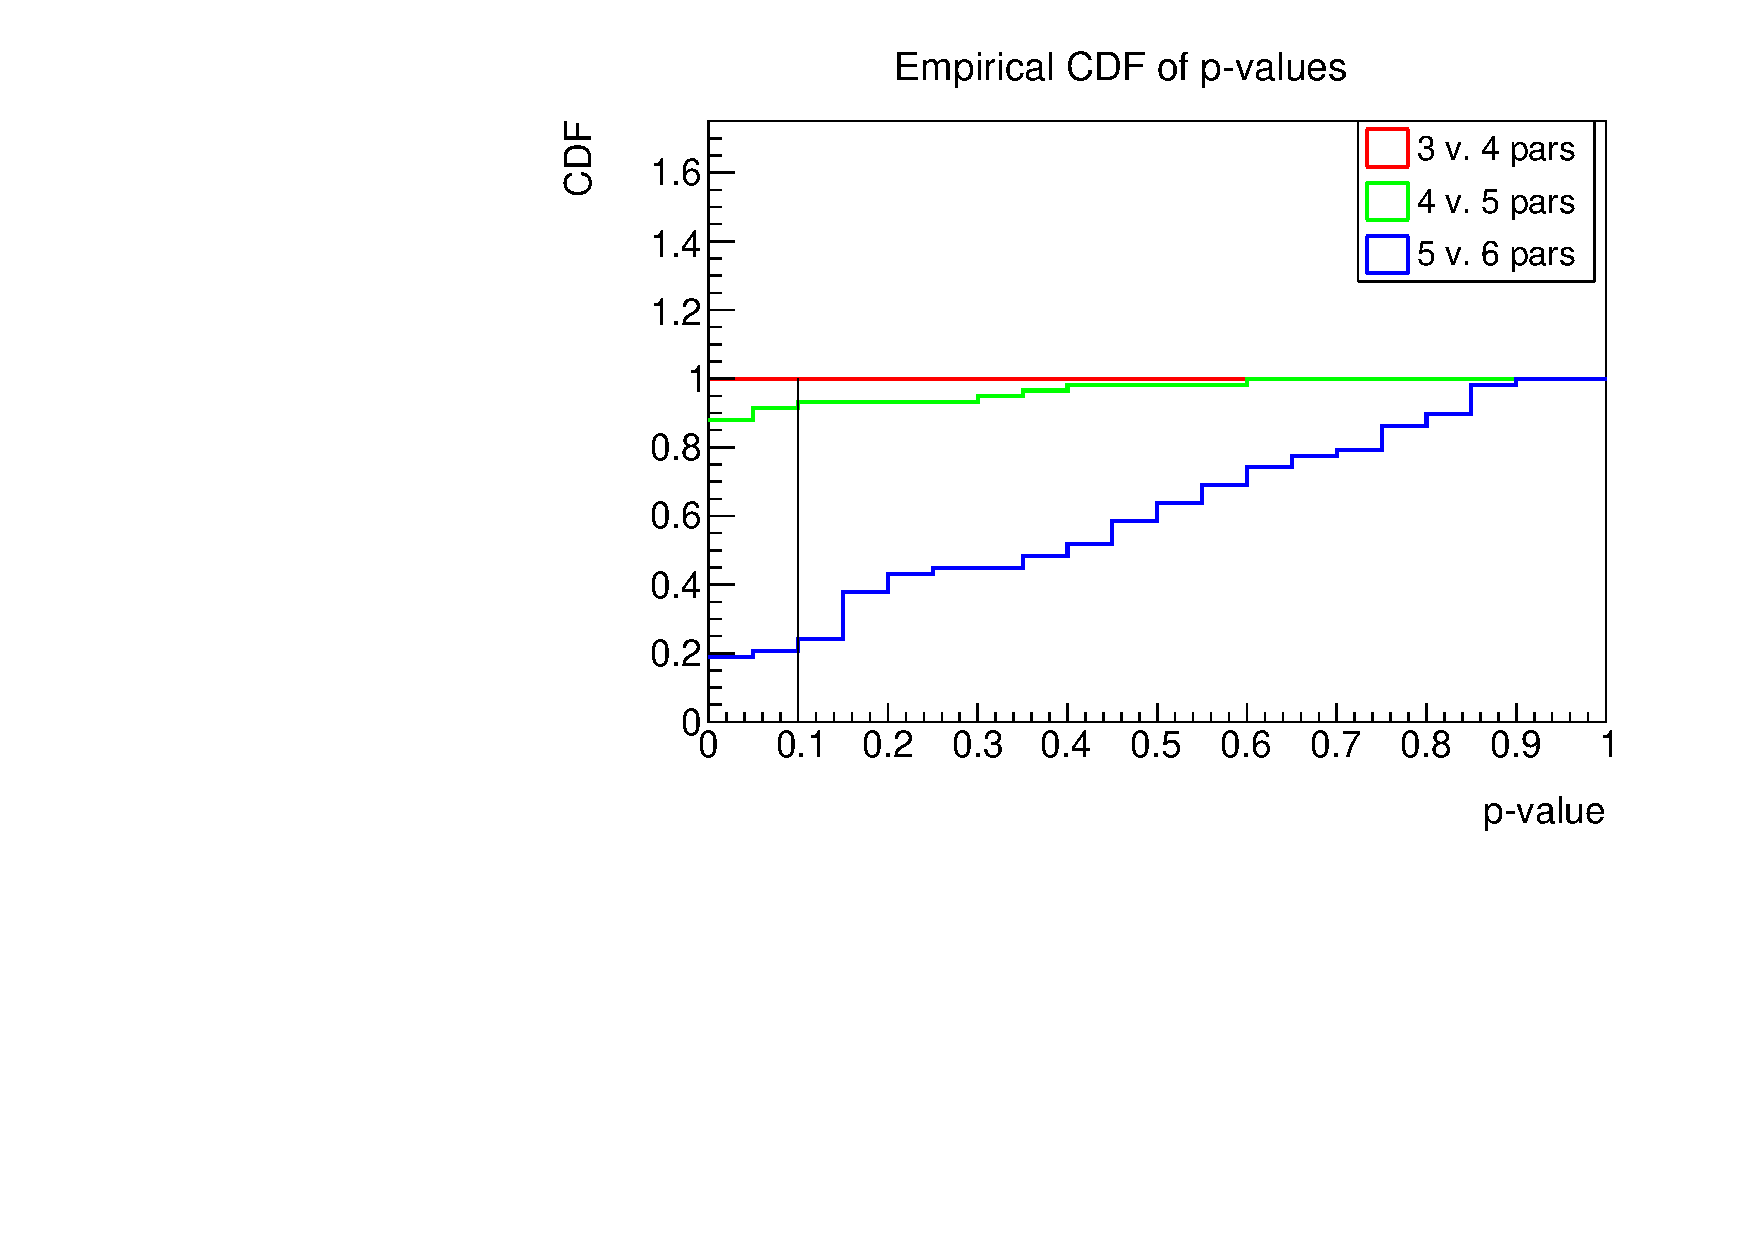
\includegraphics[width=\textwidth]{analysis/LLR_CDF_compare_polyexp.pdf}
  \caption[Empirical cumulative distribution function from the likelihood ratio test comparison for the polynomial exponential fit models.]{%
   Empirical cumulative distribution function for the observed \pvalue{}s from the likelihood ratio test for the polynomial exponential model.}
  \label{fig:LLR_CDF}
 \end{subfigure}%
 \quad
 \begin{subfigure}[t]{0.48\textwidth}
  \centering
  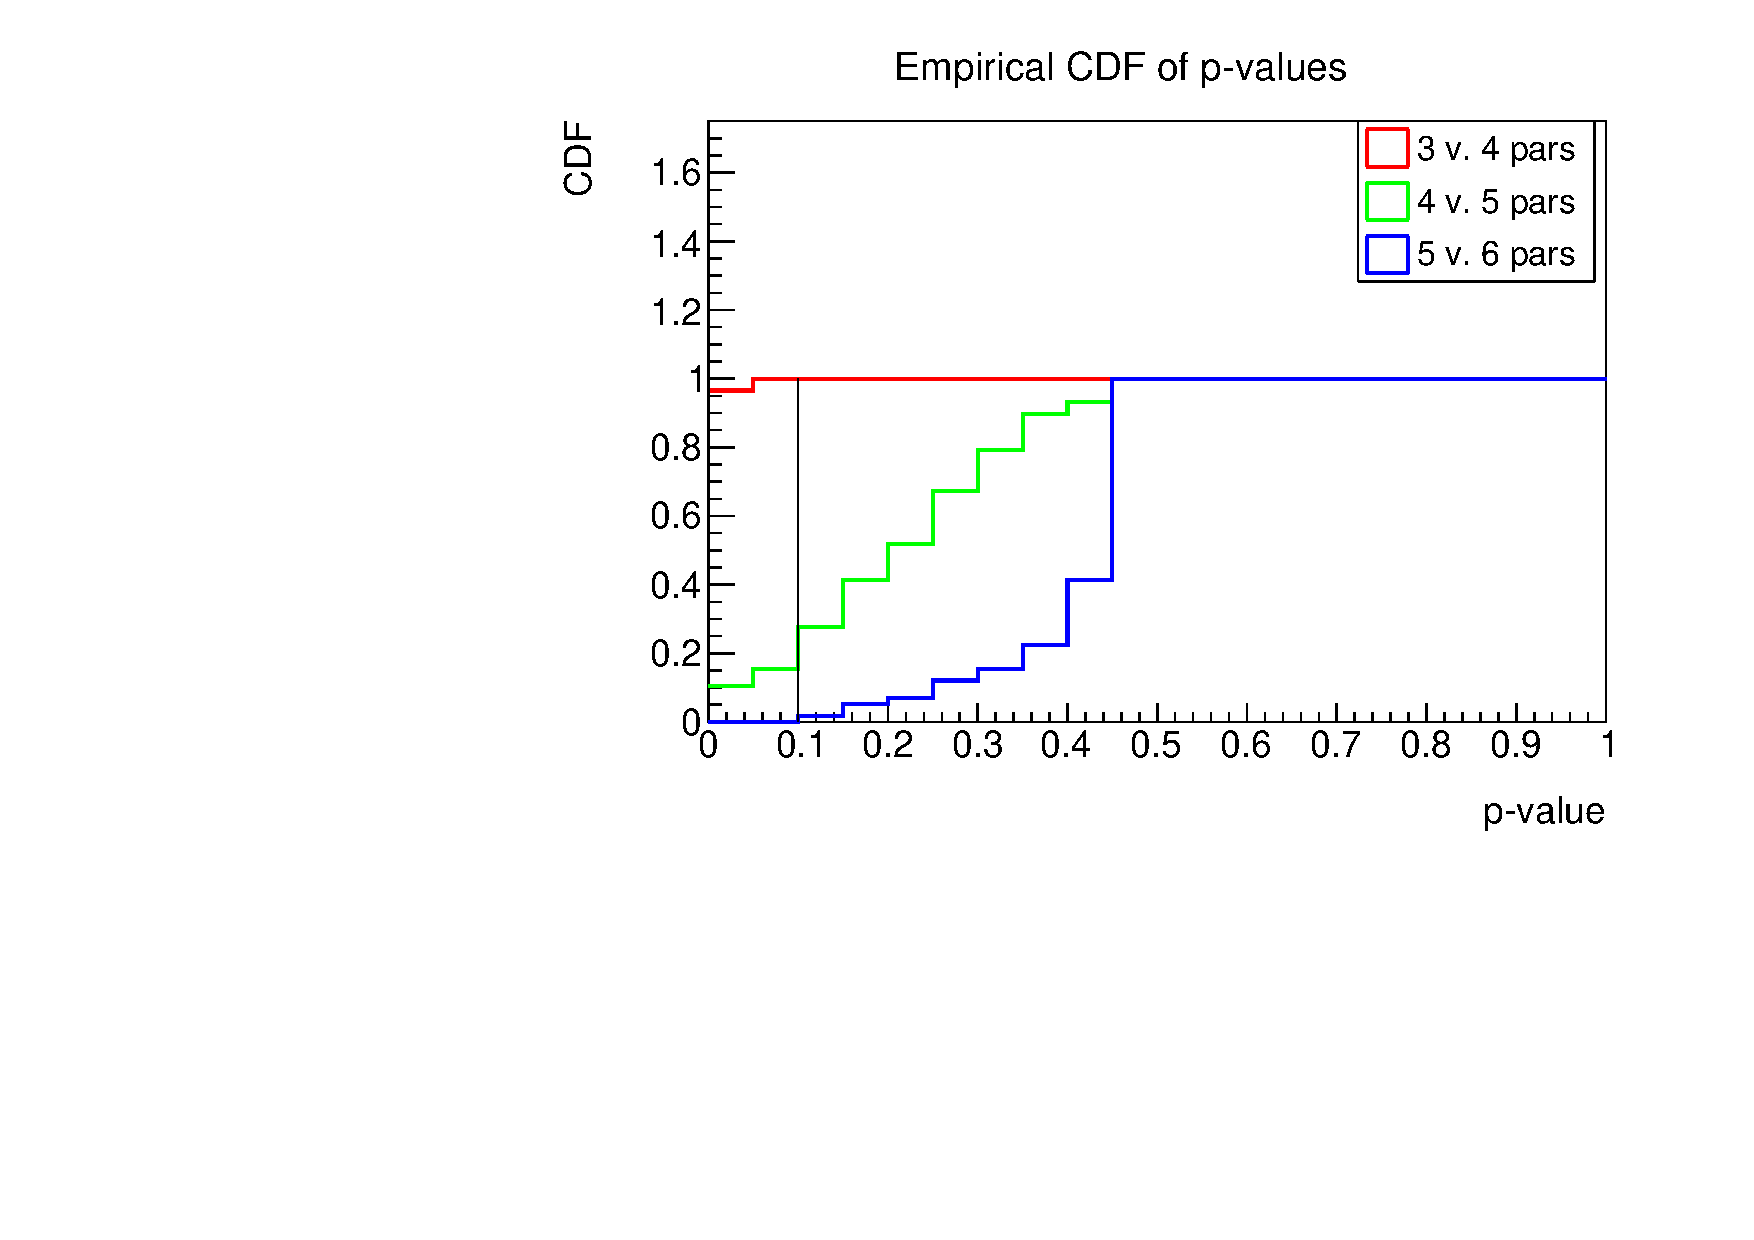
\includegraphics[width=\textwidth]{analysis/Ftest_CDF_compare_polyexp.pdf}
  \caption[Empirical cumulative distribution function from the $F$-test comparison for the polynomial exponential fit models.]{%
   Empirical cumulative distribution function for the observed \pvalue{}s from the $F$-test for the polynomial exponential model.}
  \label{fig:Ftest_CDF}
 \end{subfigure}
 \caption{Empirical cumulative distribution function for the observed \pvalue{}s for the polynomial exponential model.
  The threshold value of $\alpha=0.1$ is indicated by a vertical line.
  The likelihood ratio test favors a 5 parameter model while the $F$-test favors a 4 parameter model.}
 \label{fig:empirical_CDF_polyexp}
\end{figure}

\begin{figure}[htbp]
 \centering
 \begin{subfigure}[t]{0.48\textwidth}
  \centering
  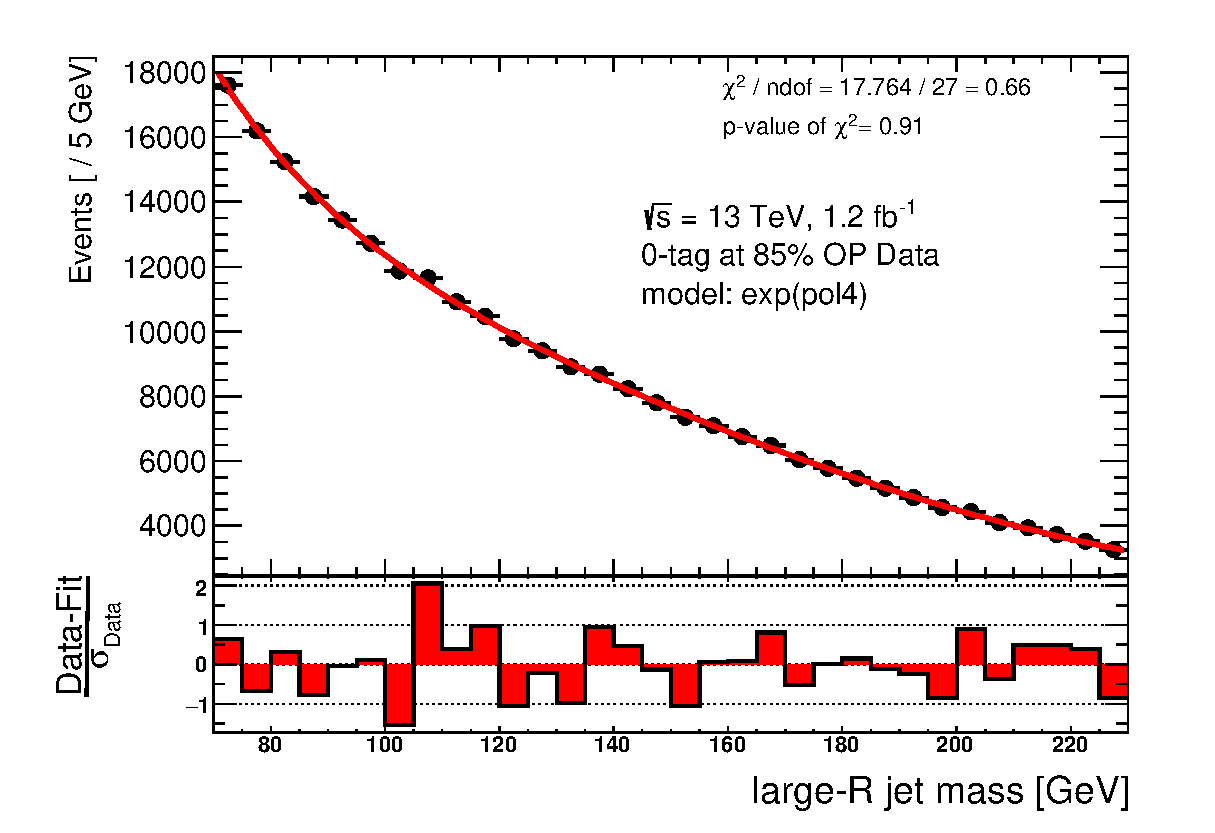
\includegraphics[width=\textwidth]{analysis/fit_5param_exp_to_CR_data_1_2ifb.eps}
  \caption[The fit of the 5 parameter polynomial exponential model to a slice of the \CRQCD{} data.]{%
   The fit of the 5 parameter polynomial exponential model to a $1.2~\ifb$ slice of the \CRQCD{} data with the resonant Monte Carlo templates subtracted.}
  \label{fig:5param_model_fit}
 \end{subfigure}%
 \quad
 \begin{subfigure}[t]{0.48\textwidth}
  \centering
  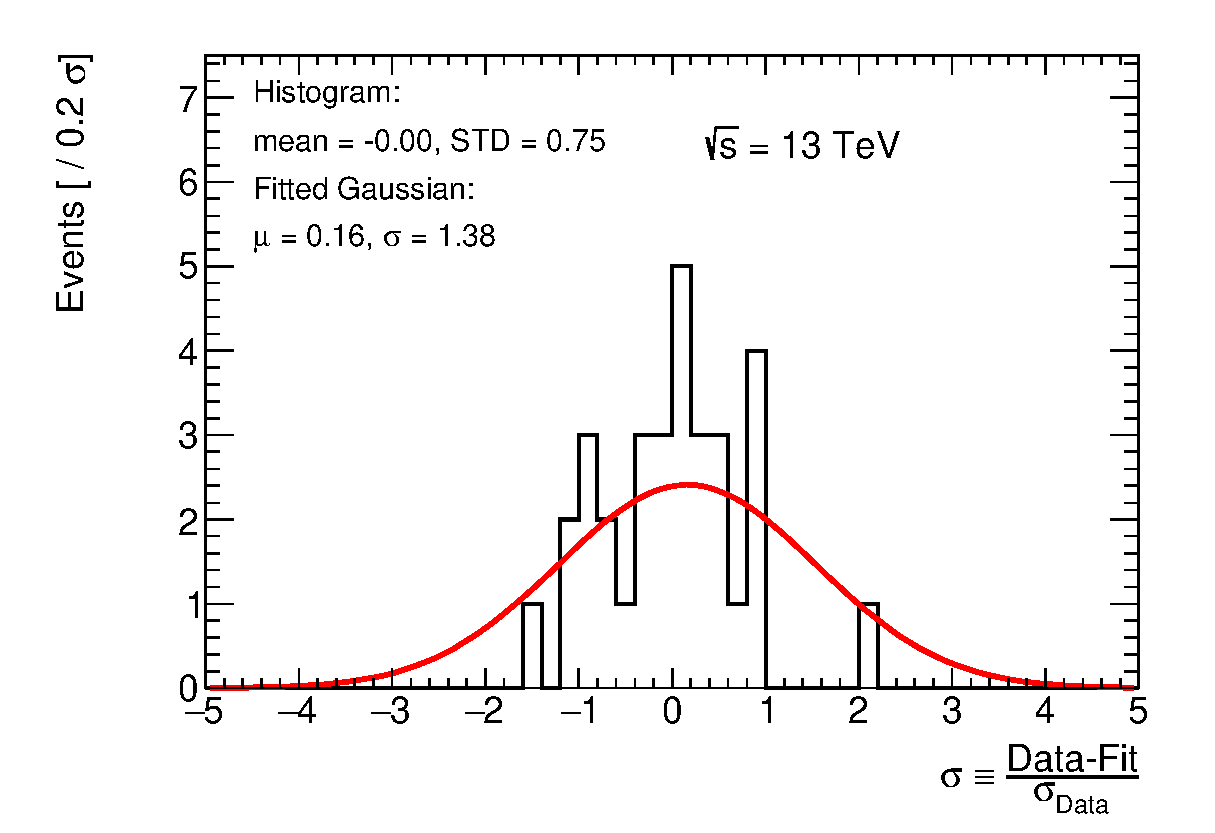
\includegraphics[width=\textwidth]{analysis/sig_dist_5param_exp_to_CR_data_1_2ifb.eps}
  \caption[Distribution of the weighted residuals of the fit.]{%
   Distribution of the weighted residuals of the fit.}
  \label{fig:5param_model_sig_dist}
 \end{subfigure}
 \caption[The fit and fit residuals of the 5 parameter polynomial exponential model to a slice of the \CRQCD{} data.]{%
  The fit of the 5 parameter polynomial exponential model to a $1.2~\ifb$ slice of the \CRQCD{} data with the resonant Monte Carlo templates subtracted.
  The fit exhibits both a low reduced $\chi^{2}$ value and a high \pvalue{} for the $\chi^{2}$ indicating a good fit.
  The distribution of the weighted residuals of the fit with a Normal distribution fitted to it.
  Though with low statistics at only 32 entries given the mass binning of $5~\GeV$, the residuals appear to be Normally distributed, which again indicates a good fit.}
 \label{fig:5param_QCD_model_fit}
\end{figure}

After fixing the number of parameters of the chosen function, the fit performance is  validated in the \CRQCD{} data slices.
The different \CRQCD{} data slices are fit with the QCD model plus the templates for the $W+\mathrm{jets}$, $Z+\mathrm{jets}$, and $\ttbar$ contributions (scaled by their cross section times the luminosity of each slice and any relevant $k$-factors).
The normalizations of the resonant background MC templates are fixed so that only the performance of the QCD model is evaluated in the fit.
From the fit results across all of the \CRQCD{} slices it is observed that the $\chi^{2}/\mathrm{ndf}$ from the individual fits follow a $\chi^{2}$ distribution, within the statistical precision given by the different data slices.

\subsection{Spurious Signal Tests}

In order to gauge how sensitive the choice of multijet model is to statistical fluctuations faking a possible signal, spurious signal tests were performed.
This is done by injecting no signal but including a signal template in the fit model and seeing if a non-zero signal strength for the signal will be fit, following the resonant MC template subtraction procedure described in \Cref{sec:models_tested}.
If the model is able to fit nonexistent signals in a statistically significant way, given the results from the \CRQCD{} fits, a systematic uncertainty will be introduced to cover the resulting bias.
If no statistically significant signal is found, no extra uncertainty is needed.
This spurious signal test is performed for the signals used in the analysis: $Z$, Higgs, $\Zprime$.

The distribution of the ratio of the fit signal strength to the uncertainty on the fit signal strength, $\mu_{\mathrm{fit}}/\sigma_{\mu\,\mathrm{fit}}$ is checked in the different \CRQCD{} slices for the different signal hypotheses.
For each signal hypothesis, a histogram containing the ratio, $\mu_{\mathrm{fit}}/\sigma_{\mu\,\mathrm{fit}}$, is made.
The means and RMS are summarized in \Cref{table:spurious_signal_test}.
From \Cref{table:spurious_signal_test}, no statistically significant deviation is observed (means of $\mu_{\mathrm{fit}}/\sigma_{\mu\,\mathrm{fit}}$ are $<1$), and given the statistical precision of the test (RMS) the deviations seem to be compatible with $0$.
It's also observed that no trend is present in the data, i.e., the deviations do not seem to be dependent on the signal hypothesis mass.
Given these results, no extra systematic uncertainty due to the modeling’s sensitivity to spurious signals from statistical fluctuations is required.

\begin{table}[htpb]
 \centering
 \caption[Summary of spurious signal tests in \CRQCD{} slices for different signal hypotheses.]{%
  Summary of spurious signal tests in \CRQCD{} slices for different signal hypotheses.}
 \begin{tabular}{@{}lrr@{}}
  \toprule
  Signal Hypothesis                   & $\mu_{\mathrm{fit}}/\sigma_{\mu\,\mathrm{fit}}$ Mean & $\mu_{\mathrm{fit}}/\sigma_{\mu\,\mathrm{fit}}$ RMS \\ \midrule
  $Z$                                 & $-0.50$                                              & $0.82$                                              \\
  Higgs                               & $0.36$                                               & $0.77$                                              \\
  $\Zprime \left(m = 100~\GeV\right)$ & $-0.42$                                              & $0.65$                                              \\
  $\Zprime \left(m = 125~\GeV\right)$ & $0.38$                                               & $0.71$                                              \\
  $\Zprime \left(m = 150~\GeV\right)$ & $0.02$                                               & $0.80$                                              \\
  $\Zprime \left(m = 175~\GeV\right)$ & $-0.38$                                              & $0.70$                                              \\
  $\Zprime \left(m = 200~\GeV\right)$ & $0.32$                                               & $0.87$                                              \\
  \bottomrule
 \end{tabular}
 \label{table:spurious_signal_test}
\end{table}

\subsection{Signal Injection Tests}\label{sec:signal_injection}

Given the choice of parametric model for the QCD multijet background a bias in the fit signal strengths of any signals can be introduced.
To determine the effect of this bias, I performed signal injection tests using a full model comprised of a parameterized QCD model and signal Monte Carlo templates scaled to the full luminosity.
The signal templates used are a $\Vjets$ template constructed from summing the contributions of the $W+\mathrm{jets}$ Monte Carlo template and the $Z+\mathrm{jets}$ Monte Carlo template with respective $k$-factors of $k_{W} = 1.28$ and $k_{Z} = 1.38$ applied~\cite{EXOT-2017-01} and a $\Zprime$ signal Monte Carlo template for a given mass hypothesis of $m_{\Zprime}\in\{100, 125, 150, 175, 200\}~\GeV$.
The $\Vjets$ template and the $\Zprime$ template both contribute one free parameter to the model which represents their respective signal strengths.
The $t\bar{t}$ Monte Carlo template is not included as it has a Gaussian constraint applied to it to be near the mean of the values determined from the $t\bar{t}$ control region studies discussed in Section~\ref{sec:ttbar}, and so is not floated in full model fit.
The full model is Poisson sampled to construct a pseudo-experiment.
The model parameters used to construct the model for the Poisson sampling are found by fitting the parameterized QCD model to the data with the resonant MC templates subtracted, and the signal templates have their signal strength parameters set to be $\mu_{V}$ and $\mu_{\Zprime}$, respectively the value of the signal strength injected.

The pseudo-experiment generated from the full model is then fit with only the parameterized QCD model.
The fit parameters from that fit are then used to initialize the QCD parameters for a fit of the fit model (i.e., the QCD model + $\Vjets$ or the full model) to the pseudo-experiment.
After the fit to the pseudo-experiment with the fit model is performed the pull for the signal strengths for the injected signals (i.e., $\Vjets$ or $\Vjets$ and the $\Zprime$) is calculated, where the pull is defined as
\begin{equation}
 \mathrm{pull} = \frac{\mu_{\mathrm{fit}} - \mu_{\mathrm{injected}}}{\sigma_{\mu\textrm{ fit}}}.
 \label{eq:pull}
\end{equation}
This process of generating a pseudo-experiment, fitting with the fit model, and then calculating the pull for the signal components is repeated for $10,000$ trials.
If the gradient minimizer does not converge during the fit then the trial is discarded.
For the QCD multijet models used in the analysis all trials converged.
The pulls for each pseudo-experiment are then histogrammed and a Normal distribution is fit to the histogram.
If the fit is unbiased, then one should expect the pulls to be Normally distributed with a mean of 0 and width of 1,
\[
 \textrm{pulls} \sim \mathcal{N}\left(\mu=0, \sigma=1\right).
\]
The deviation of the fit Normal distribution's mean from $0$ is then an indicator of the bias of the pull given the choice of QCD model.
The number of trials was chosen to be $10,000$ as for an unbiased fit that gives a uncertainty on the distribution mean of
\[
 \left.\sigma_{\hat{\mu}} = \frac{\sigma}{\sqrt{\textrm{N trials}}}\right|_{\sigma = 1, \textrm{N trials}=10,000} = 0.01.
\]

\subsubsection{1D Tests}
To check the effects of the fit of the $\Vjets$ in the presence of an exotic signal, signal injection tests were performed with a fit model comprised of the parameterized QCD model + $\Vjets$ signal template.
For these tests the $\Vjets$ template was injected with a signal strength of $\mu_{V} = 1$, and the $\Zprime$ template with signal strength of $\mu_{\Zprime} = \mu \in \left\{0, 0.2, 0.5, 0.8, 1, 2, 3, 4, 5\right\}$.

To check the effect of shape differences between generator choice on the bias the signal injection tests were performed with the components of the toy from the $\Vjets$ sampled from a Monte Carlo template generated with \textsc{Sherpa} while the $\Vjets$ template that was used in the fit model was generated with \textsc{Herwig} with the same normalization as the \textsc{Sherpa} template.
\Cref{fig:pulls_summary_Herwig} shows the pull distributions for all $\Zprime$ mass hypotheses of $m_{\Zprime} \in \left\{100, 125, 150, 175, 200\right\}~\GeV$ and all injected signal strengths of $\mu_{\Zprime} = \mu \in \left\{0, 0.2, 0.5, 0.8, 1, 2, 3, 4, 5\right\}$ with $\mu_{V} = 1$.
The pulls means show large deviations from $0$ indicating a strong bias when trying to fit the toys drawn from \textsc{Sherpa} templates with a \textsc{Herwig} template component in the fit model.
This shows that there is a substantial difference in shape between the \textsc{Sherpa} templates and the \textsc{Herwig} templates, providing motivation for a systematic uncertainty associated with the generator choice for the $W+\mathrm{jets}$ and $Z+\mathrm{jets}$ templates.

\begin{figure}[htbp]
 \centering
 \begin{subfigure}[t]{0.48\textwidth}
  \centering
  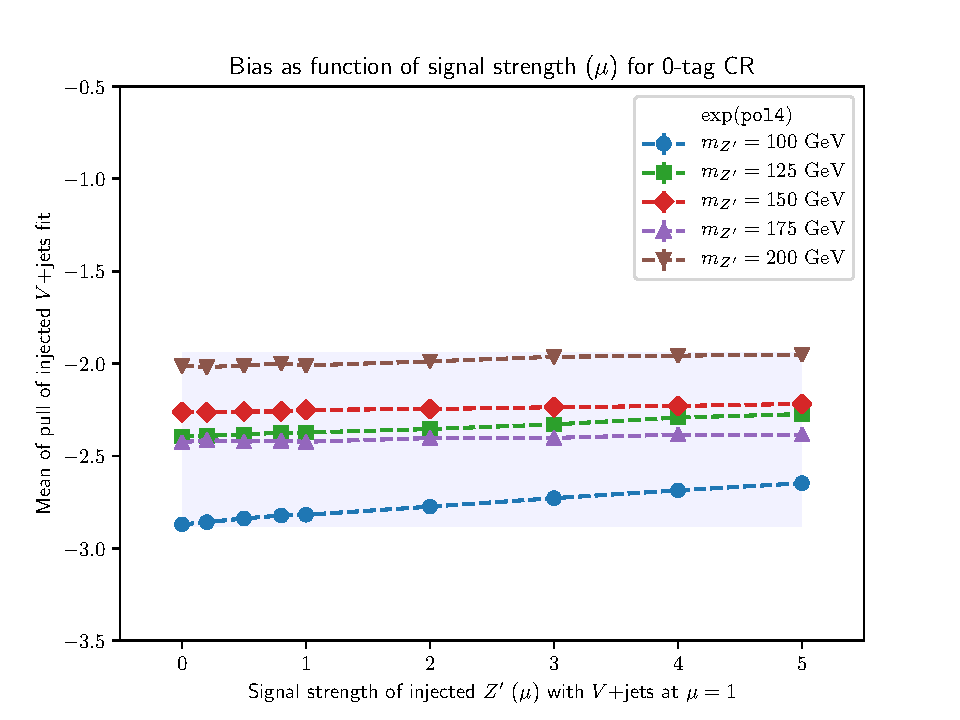
\includegraphics[width=\textwidth]{analysis/Herwig_pull_means_CR_Vjets.pdf}
  \caption[The distribution of the pull mean for $\Vjets$ and signal strengths vs. the injected $\Zprime$ signal strength.]{%
   The distribution of the pull mean for $\Vjets$ and signal strengths vs. the injected $\Zprime$ signal strength.}
  \label{fig:pulls_Vjets_Herwig}
 \end{subfigure}%
 \quad
 \begin{subfigure}[t]{0.48\textwidth}
  \centering
  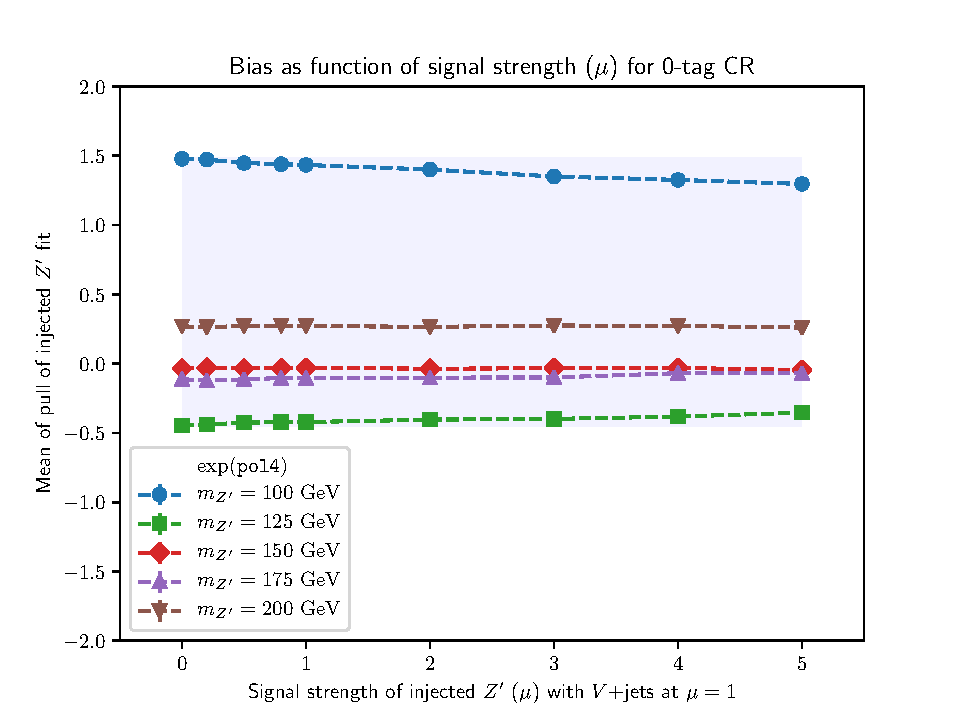
\includegraphics[width=\textwidth]{analysis/Herwig_pull_means_CR_Zprime.pdf}
  \caption[The distribution of the pull mean for $\Zprime$ signal strengths vs. the injected $\Zprime$ signal strength.]{%
   The distribution of the pull mean for $\Zprime$ signal strengths vs. the injected $\Zprime$ signal strength.}
  \label{fig:pulls_Zprime_Herwig}
 \end{subfigure}
 \caption[The distribution of the pull mean for fit signal strengths vs. the injected $\Zprime$ signal strength with \textsc{Herwig} Monte Carlo templates.]{%
  The distribution of the pull mean for fit signal strengths vs. the injected $\Zprime$ signal strength $\mu_{\Zprime}$ for $\mu_{\Zprime} = \mu \in \left\{0, 0.2, 0.5, 0.8, 1, 2, 3, 4, 5\right\}$ with $\mu_{V} = 1$ using a full fit model with a $\Vjets$ Monte Carlo template generated using \textsc{Herwig} and with a $\Zprime$ mass hypothesis $m_{\Zprime}$ for
  $m_{\Zprime} \in \left\{100, 125, 150, 175, 200\right\}~\GeV$.
  The lightly shaded rectangular region encloses the extrema of the pull means and their statistical uncertainties, showing large biases.
  The dashed straight lines are meant only as visual guides, and are not to be treated as linear interpolations between signal strengths.}
 \label{fig:pulls_summary_Herwig}
\end{figure}

Given the statistical precision of the Monte Carlo templates, scaling them to correspond to the observed luminosity results in statistical fluctuations in the tails of the templates to become enlarged into apparent features.
This is not desirable, as these features are not physical, and so the Monte Carlo templates were smoothed for use in fitting by modeling them with functional forms fit to data.
To check the bias associated with fits using models that contain smoothed Monte Carlo templates generated from \textsc{Sherpa}, the signal injection tests were performed again.
\Cref{fig:pulls_summary_smoothed_Sherpa} shows the pull distributions for all $\Zprime$ mass hypotheses of $m_{\Zprime} \in \left\{100, 125, 150, 175, 200\right\}~\GeV$ and all injected signal strengths of $\mu_{\Zprime} = \mu \in \left\{0, 0.2, 0.5, 0.8, 1, 2, 3, 4, 5\right\}$ with $\mu_{V} = 1$.
As the pull means are contained within a $\pm 3\%$ window of the statistical uncertainties of the fit signal strength, then for a QCD model of a 5 parameter polynomial exponential the fit bias is small enough that an additional systematic uncertainty for the choice of QCD model parameterization is unnecessary.

To check the bias for a signal model of a Higgs boson the signal injection tests with smoothed \textsc{Sherpa} Monte Carlo templates were run again, but with a smoothed Higgs template for a signal model instead of a $\Zprime$.
\Cref{fig:pulls_summary_Higgs_smoothed_Sherpa} shows the pull distributions for injected signal strengths of the Higgs of $\mu_{H} = \mu \in \left\{0, 0.2, 0.5, 0.8, 1, 2, 3, 4, 5\right\}$ with $\mu_{V} = 1$.
The pull means being well contained within a $\left[-3,+2\right]\%$ window of the statistical uncertainties of the fit signal strength gives additional evidence that for a QCD model of a 5 parameter polynomial exponential the fit bias is small enough that an additional systematic uncertainty for the choice of QCD model parameterization is unnecessary, regardless of signal model chosen.

\begin{figure}[htbp]
 \centering
 \begin{subfigure}[t]{0.48\textwidth}
  \centering
  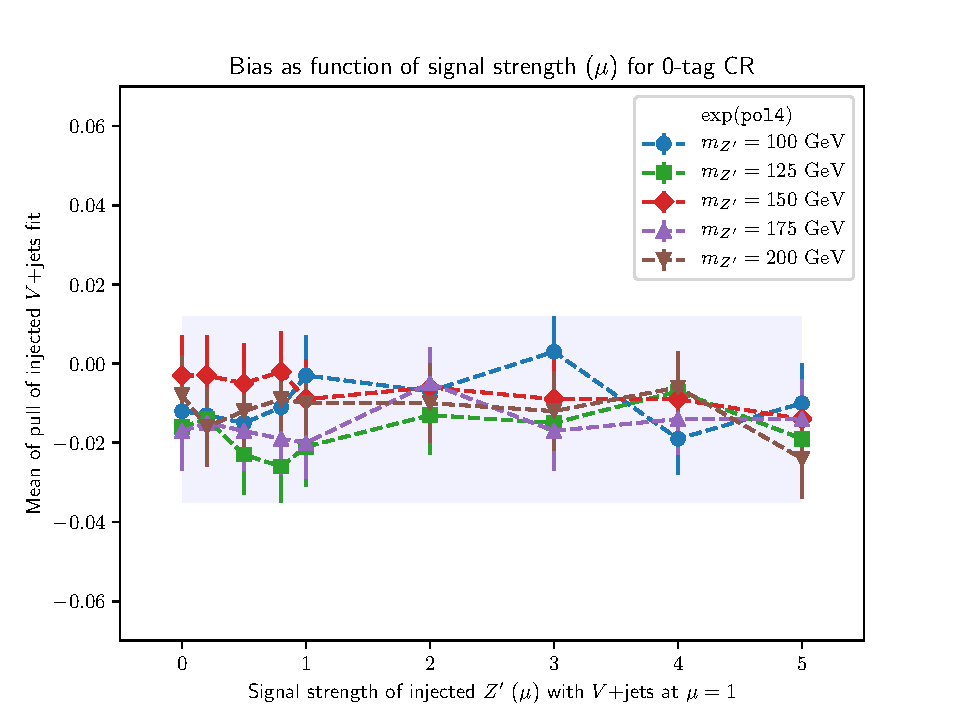
\includegraphics[width=\textwidth]{analysis/smoothed_Sherpa_pull_means_CR_Vjets.pdf}
  \caption[The distribution of the pull mean for $\Vjets$ and signal strengths vs. the injected $\Zprime$ signal strength.]{%
   The distribution of the pull mean for $\Vjets$ and signal strengths vs. the injected $\Zprime$ signal strength.}
  \label{fig:pulls_Vjets_Sherpa}
 \end{subfigure}%
 \quad
 \begin{subfigure}[t]{0.48\textwidth}
  \centering
  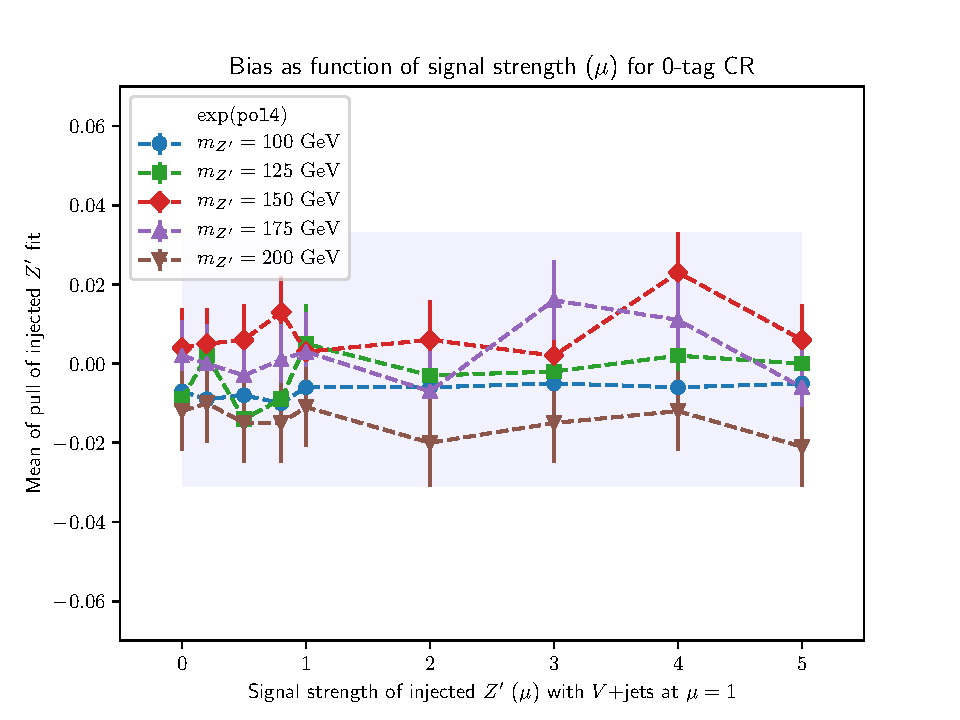
\includegraphics[width=\textwidth]{analysis/smoothed_Sherpa_pull_means_CR_Zprime.pdf}
  \caption[The distribution of the pull mean for $\Zprime$ signal strengths vs. the injected $\Zprime$ signal strength.]{%
   The distribution of the pull mean for $\Zprime$ signal strengths vs. the injected $\Zprime$ signal strength.}
  \label{fig:pulls_Zprime_Sherpa}
 \end{subfigure}
 \caption[The distribution of the pull mean for fit signal strengths vs. the injected $\Zprime$ signal strength with \textsc{Sherpa} Monte Carlo templates.]{%
  The distribution of the pull mean for fit signal strengths vs. the injected $\Zprime$ signal strength $\mu_{\Zprime}$ for $\mu_{\Zprime} = \mu \in \left\{0, 0.2, 0.5, 0.8, 1, 2, 3, 4, 5\right\}$ with $\mu_{V} = 1$ using a full fit model with smoothed Monte Carlo templates generated using \textsc{Sherpa} and with a $\Zprime$ mass hypothesis $m_{\Zprime}$ for
  $m_{\Zprime} \in \left\{100, 125, 150, 175, 200\right\}~\GeV$.
  The lightly shaded rectangular region encloses the extrema of the pull means and their statistical uncertainties, showing that the range of bias on the pulls are within a few percent of the statistical uncertainties on the fit signal strengths.
  The dashed straight lines are meant only as visual guides, and are not to be treated as linear interpolations between signal strengths.}
 \label{fig:pulls_summary_smoothed_Sherpa}
\end{figure}

\begin{figure}[htbp]
 \centering
 \begin{subfigure}[t]{0.48\textwidth}
  \centering
  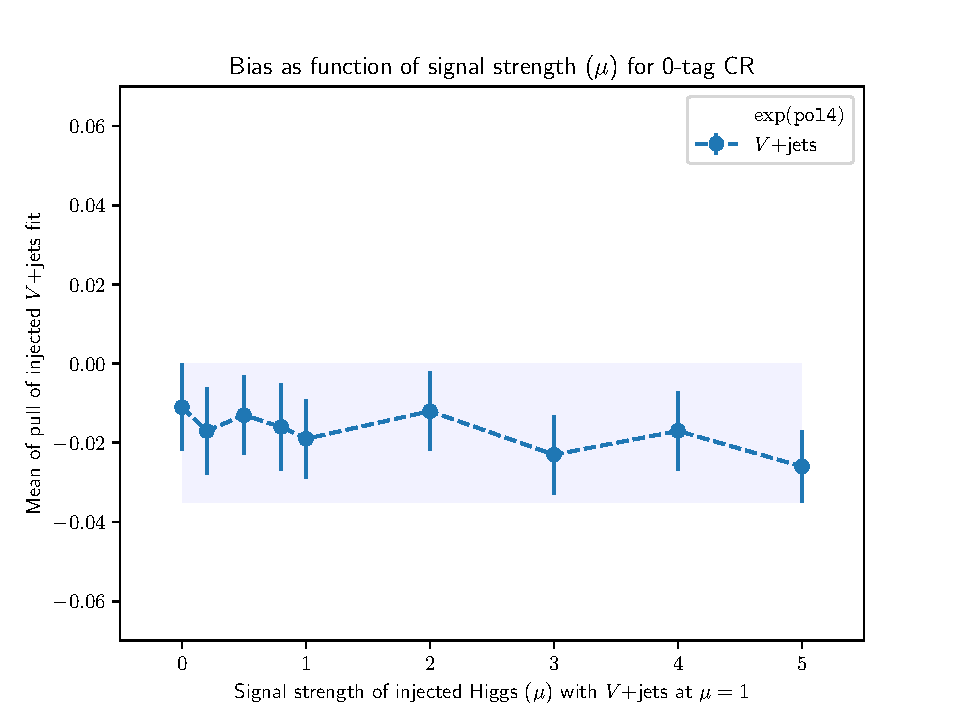
\includegraphics[width=\textwidth]{analysis/smoothed_Sherpa_pull_means_CR_Vjets_for_Higgs.pdf}
  \caption[The distribution of the pull mean for $\Vjets$ and signal strengths vs. the injected Higgs signal strength.]{%
   The distribution of the pull mean for $\Vjets$ and signal strengths vs. the injected Higgs signal strength.}
  \label{fig:pulls_Vjets_smoothed_Sherpa}
 \end{subfigure}%
 \quad
 \begin{subfigure}[t]{0.48\textwidth}
  \centering
  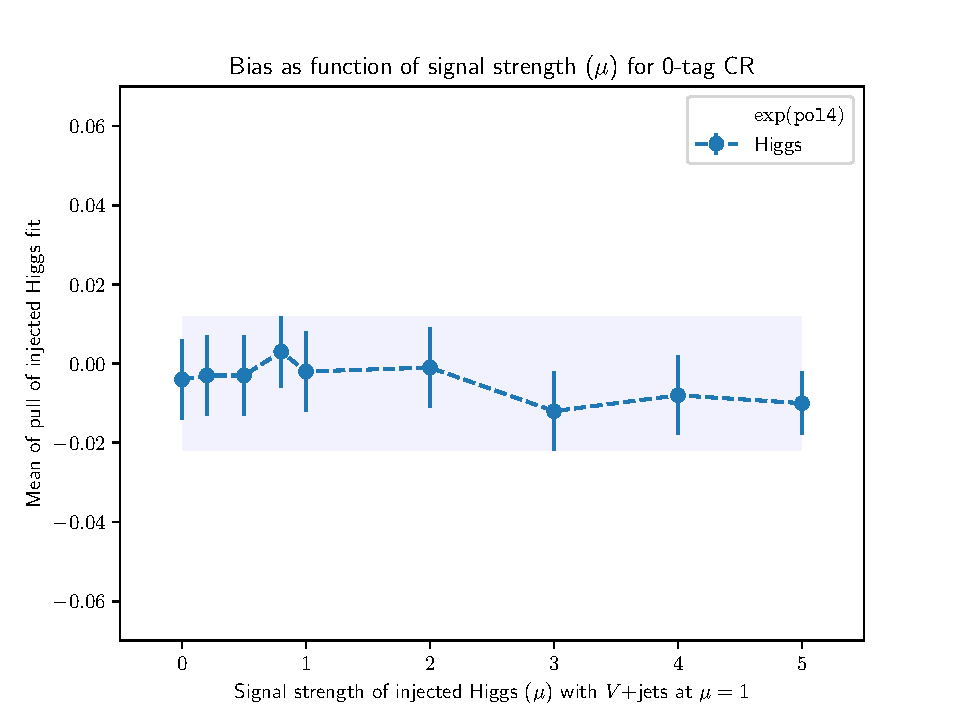
\includegraphics[width=\textwidth]{analysis/smoothed_Sherpa_pull_means_CR_Higgs.pdf}
  \caption[The distribution of the pull mean for Higgs signal strengths vs. the injected Higgs signal strength.]{%
   The distribution of the pull mean for Higgs signal strengths vs. the injected Higgs signal strength.}
  \label{fig:pulls_Higgs_smoothed_Sherpa}
 \end{subfigure}
 \caption[The distribution of the pull mean for fit signal strengths vs. the injected Higgs signal strength.]{%
  The distribution of the pull mean for fit signal strengths vs. the injected Higgs signal strength $\mu_{H}$ for $\mu_{H} = \mu \in \left\{0, 0.2, 0.5, 0.8, 1, 2, 3, 4, 5\right\}$ with $\mu_{V} = 1$ using a full fit model with smoothed Monte Carlo templates generated using \textsc{Sherpa} for the $\Vjets$ and Higgs.
  The lightly shaded rectangular region encloses the extrema of the pull means and their statistical uncertainties, showing that the range of bias on the pulls are within a few percent of the statistical uncertainties on the fit signal strengths.
  The dashed straight lines are meant only as visual guides, and are not to be treated as linear interpolations between signal strengths.}
 \label{fig:pulls_summary_Higgs_smoothed_Sherpa}
\end{figure}

\subsubsection{2D Tests}

To check the effects of the interaction of the $\Vjets$ and $\Zprime$ signal templates being fit together the signal injection tests were performed with a fit model comprised of the parameterized QCD model + $\Vjets$ signal template + the $\Zprime$ signal template.
\Cref{fig:pulls_Zprime100_mu1} shows the pull distributions for an example of a $\Zprime$ mass hypothesis of $m_{\Zprime}=100~\GeV$ and injected signal strengths of $\mu_{V} = \mu_{\Zprime} = \mu = 1$.
The procedure is then repeated for injected signal strengths $\mu \in \left\{0, 0.2, 0.5, 0.8, 1, 2, 3, 4, 5\right\}$ for each $\Zprime$ mass hypothesis.
Figure~\ref{fig:pulls_summary} shows the pull distributions for all $\Zprime$ mass hypotheses of $m_{\Zprime} \in \left\{100, 125, 150, 175, 200\right\}~\GeV$ and all injected signal strengths of $\mu_{V} = \mu_{\Zprime} = \mu \in \left\{0, 0.2, 0.5, 0.8, 1, 2, 3, 4, 5\right\}$.
As the pull means are contained within a $\left[-5,+3\right]\%$ window of the statistical uncertainties of the fit signal strength, then for a QCD model of a 5 parameter polynomial exponential the fit bias is small enough that an additional systematic uncertainty for the choice of QCD model parameterization is unnecessary.

\begin{figure}[htbp]
 \centering
 \begin{subfigure}[t]{0.48\textwidth}
  \centering
  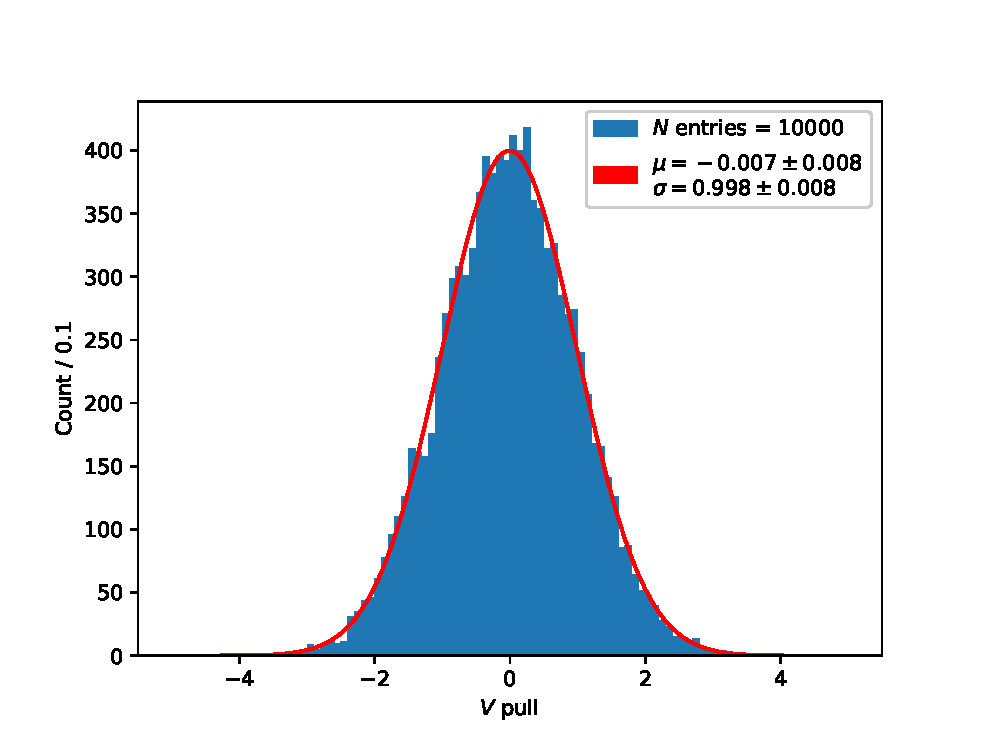
\includegraphics[width=\textwidth]{analysis/Vjets_pull_hist_Zprime100_mu1.eps}
  \caption[The pull distributions for the fit signal strength for $\Vjets$ using a full model with a $\Zprime$ mass hypothesis of $m_{\Zprime}=100~\GeV$.]{%
   The pull distributions for the fit signal strength for $\Vjets$ using a full model with a $\Zprime$ mass hypothesis of $m_{\Zprime}=100~\GeV$ and injected signal strengths of $\mu_{V} = \mu_{\Zprime} = \mu = 1$.}
  \label{fig:Vjets_pulls_Zprime100_mu1}
 \end{subfigure}%
 \quad
 \begin{subfigure}[t]{0.48\textwidth}
  \centering
  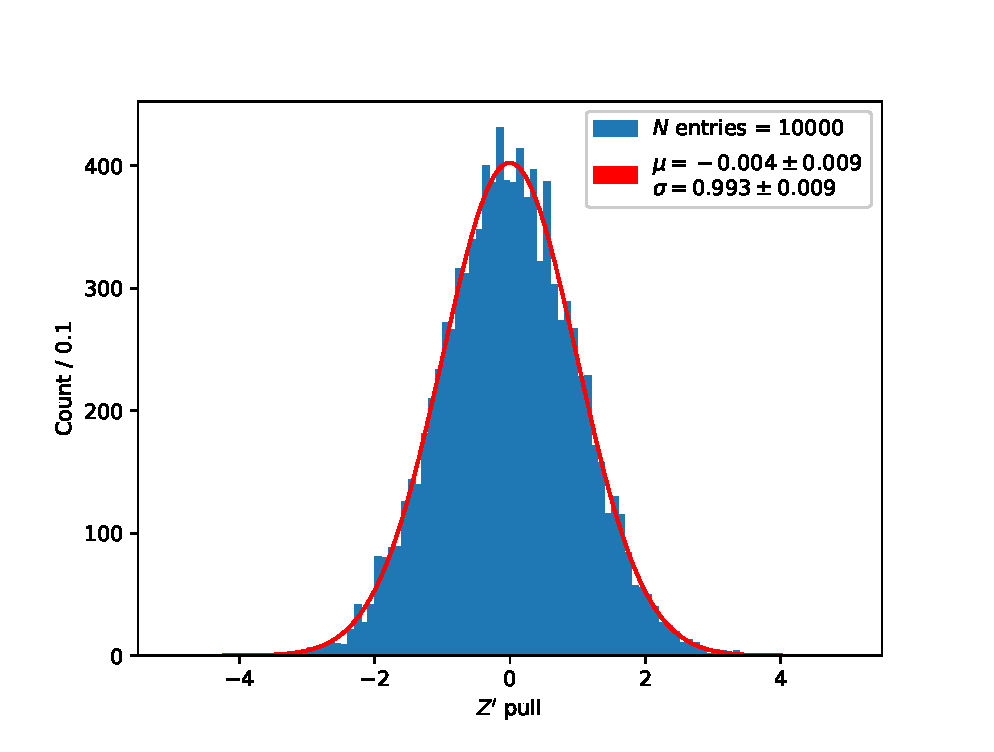
\includegraphics[width=\textwidth]{analysis/Zprime_pull_hist_Zprime100_mu1.eps}
  \caption[The pull distributions for the fit signal strengths for $\Zprime$ using a full model with a $\Zprime$ mass hypothesis of $m_{\Zprime}=100~\GeV$.]{%
   The pull distributions for the fit signal strengths for $\Zprime$ using a full model with a $\Zprime$ mass hypothesis of $m_{\Zprime}=100~\GeV$ and injected signal strengths of $\mu_{V} = \mu_{\Zprime} = \mu = 1$.}
  \label{fig:Zprime_pulls_Zprime100_mu1}
 \end{subfigure}
 \caption[The pull distributions for the fit signal strengths using a full model with a $\Zprime$ mass hypothesis of $m_{\Zprime}=100~\GeV$ and injected signal strengths of $\mu_{V} = \mu_{\Zprime} = \mu = 1$.]{%
  The pull distributions for the fit signal strengths using a full model with a $\Zprime$ mass hypothesis of $m_{\Zprime}=100~\GeV$ and injected signal strengths of $\mu_{V} = \mu_{\Zprime} = \mu = 1$.
  A Gaussian is fit to the pull distributions with the best fit results for the Gaussian's mean and standard deviation shown on the plot with their respective uncertainties.}
 \label{fig:pulls_Zprime100_mu1}
\end{figure}

\begin{figure}[htbp]
 \centering
 \begin{subfigure}[t]{0.48\textwidth}
  \centering
  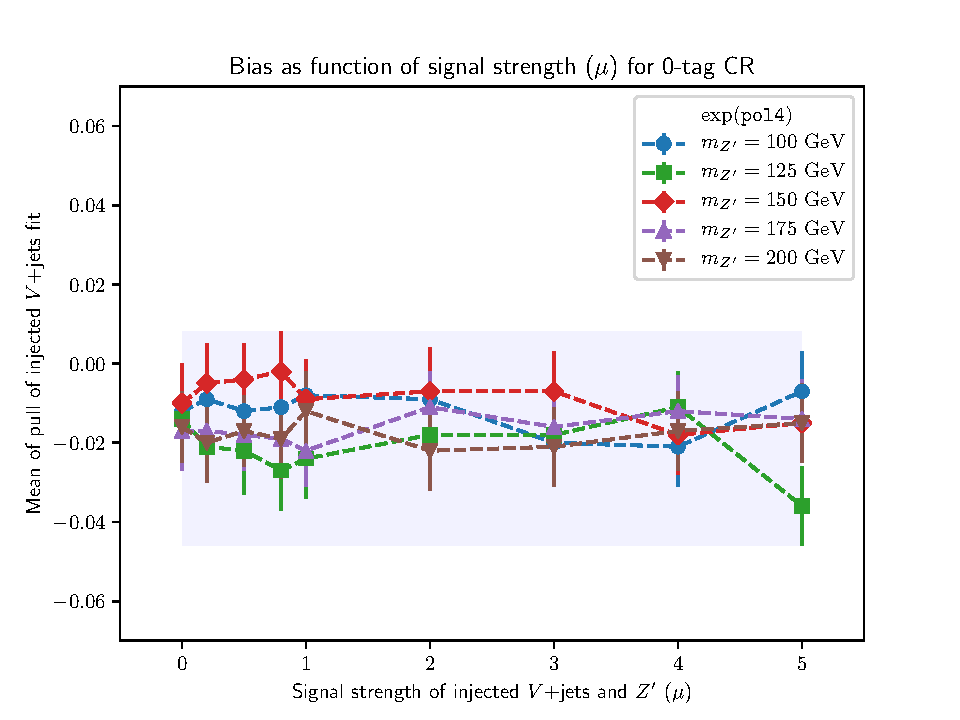
\includegraphics[width=\textwidth]{analysis/pull_means_CR_Vjets.pdf}
  \caption[The distribution of the pull mean for $\Vjets$ signal strength vs. the injected signal strength $\mu$ using a full model with a $\Zprime$ mass hypothesis $m_{\Zprime}$.]{%
   The distribution of the pull mean for $\Vjets$ signal strength vs. the injected signal strength $\mu$ using a full model with a $\Zprime$ mass hypothesis $m_{\Zprime}$.}
  \label{fig:pull_means_CR_Vjets}
 \end{subfigure}%
 \quad
 \begin{subfigure}[t]{0.48\textwidth}
  \centering
  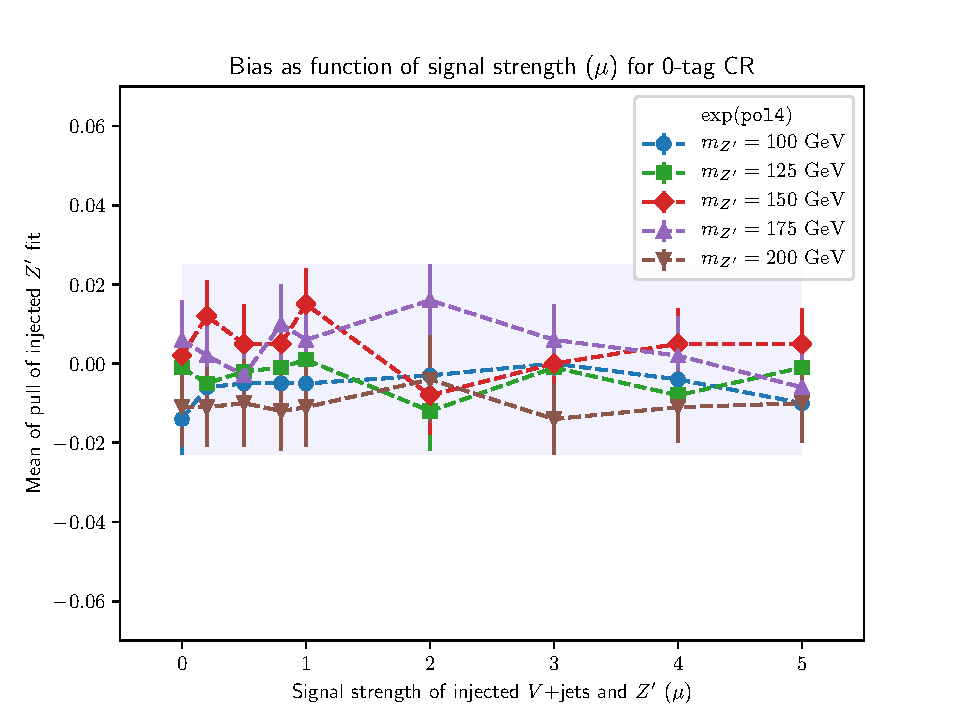
\includegraphics[width=\textwidth]{analysis/pull_means_CR_Zprime.pdf}
  \caption[The distribution of the pull mean for $\Zprime$ signal strength vs. the injected signal strength $\mu$ using a full model with a $\Zprime$ mass hypothesis $m_{\Zprime}$.]{%
   The distribution of the pull mean for $\Zprime$ signal strength vs. the injected signal strength $\mu$ using a full model with a $\Zprime$ mass hypothesis $m_{\Zprime}$.}
  \label{fig:pull_means_CR_Zprime}
 \end{subfigure}
 \caption[The distribution of the pull mean for fit signal strengths vs. the injected signal strength $\mu$ using a full model with a $\Zprime$ mass hypothesis $m_{\Zprime}$.]{%
  The distribution of the pull mean for fit signal strengths vs. the injected signal strength $\mu$ for $\mu \in \left\{0, 0.2, 0.5, 0.8, 1, 2, 3, 4, 5\right\}$ using a full model with a $\Zprime$ mass hypothesis $m_{\Zprime}$ for $m_{\Zprime} \in \left\{100, 125, 150, 175, 200\right\}~\GeV$.
  The lightly shaded rectangular region encloses the extrema of the pull means and their statistical uncertainties, showing that the range of bias on the pulls are within a few percent of the statistical uncertainties on the fit signal strengths.
  The dashed straight lines are meant only as visual guides, and are not to be treated as linear interpolations between signal strengths.}
 \label{fig:pulls_summary}
\end{figure}

\subsubsection{Alternate QCD Model}

The alternative function choice, the Formal Laurent series \Cref{eq:formal_laurent}, is also tested.
\Cref{fig:likelihood_ratio_test_laurent} shows the results of the two statistical test being applied to the Formal Laurent series family of functions.
Given the \pvalue{}s of the likelihood ratio test and $F$-test are $p < \left(\alpha=0.1\right)$ in the comparison between the 3 and 4 parameter models the 4 parameter model is selected as giving a statistically significant improvement to the fit.
Given the large \pvalue{}s observed between the 5 and 6 parameter model, $p > 0.1$, the addition of a 6th parameter to the model does not contribute to a significant improvement in the fit.
However, when comparing the 4 and 5 parameter models it is seen that there is contention between the likelihood ratio test and $F$-test, as summarized in \Cref{table:stat_test_parameters_laurent}.
To attempt to resolve the contention, the two statistical tests for the Formal Laurent series family of functions are repeated for all \CRQCD{} data slices.
The relative frequencies of the observed \pvalue{}s for the tests are iteratively summed, as seen in \Cref{fig:empirical_CDF_laurent}, producing an empirical cumulative distribution function for the test \pvalue{}s.
It is seen that for the \emph{a priori} threshold of $\alpha=0.1$ that in a non-negligible fraction of the cases the likelihood ratio test favors a 5 parameter model ($\textrm{CDF}_{4\textrm{v.}5}\left(0.1\right) > 0.4$) while in all cases the $F$-test favors a 4 parameter model.
As the contention remains, the 5 parameter model is conservatively chosen to model the shape of the QCD background distribution.
\Cref{fig:5param_QCD_model_fit_laurent} shows the result of the fit in the original data slice with the selected 5 parameter QCD model.
As in \Cref{sec:model_selection}, the \CRQCD{} slices were fit with contributions for $\Vjets$ and $\ttbar$ fixed to their SM normalizations times the appropriate $k$-factors.
The $\chi^2/\mathrm{ndf}$ distribution from the data slices fits is consistent with the expected distribution.
Given the Formal Laurent series also robustly models the multijet continuum distribution it is used to evaluate a systematic uncertainty from model choice, as described in \Cref{sec:systematic_uncertainties}.

\begin{figure}[htbp]
 \centering
 \begin{subfigure}[t]{0.333\textwidth}
  \centering
  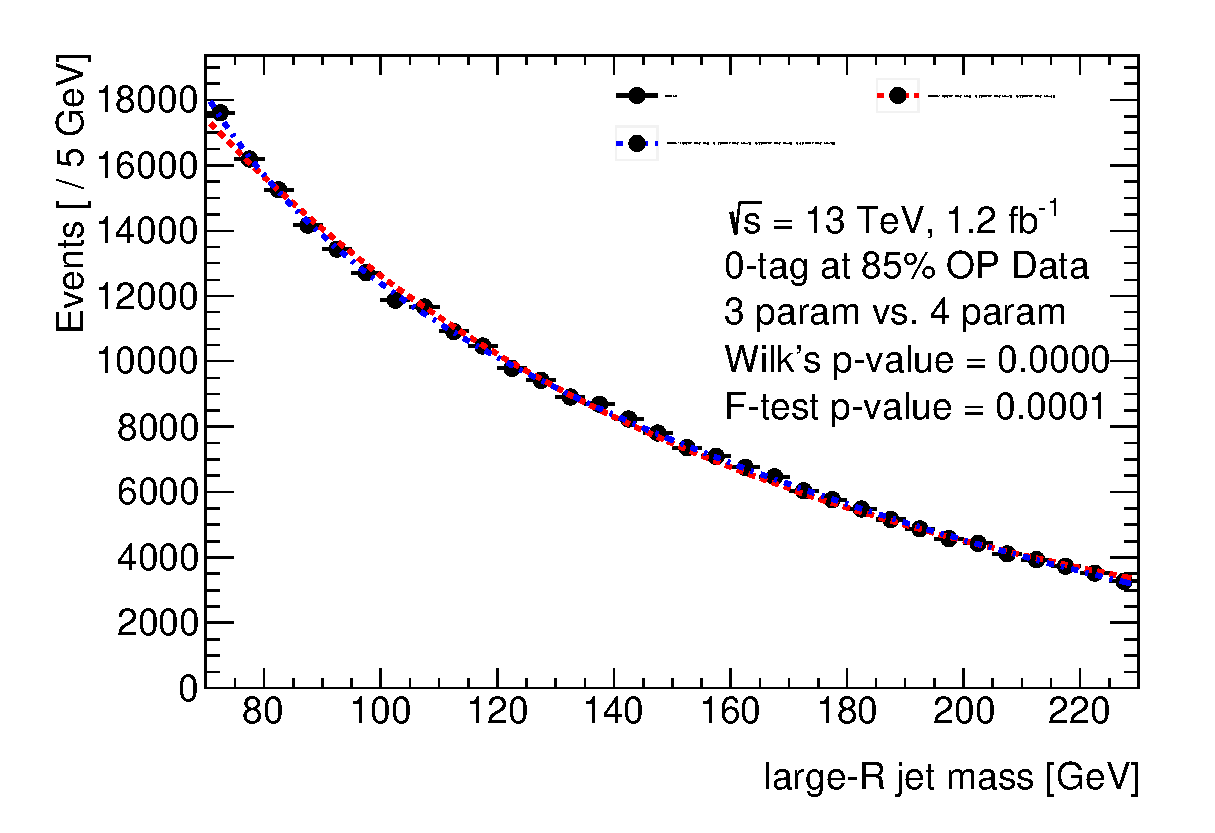
\includegraphics[width=\textwidth]{analysis/stat_test_laurent_3_v_4params_CR_data.eps}
  \caption[Comparison of the Formal Laurent fit models with 3 and 4 parameters.]{%
   Statistical test results of comparison of the Formal Laurent fit models with 3 and 4 parameters.}
  \label{fig:stat_test_laurent_3_v_4params_CR_data}
 \end{subfigure}%
 ~
 \begin{subfigure}[t]{0.333\textwidth}
  \centering
  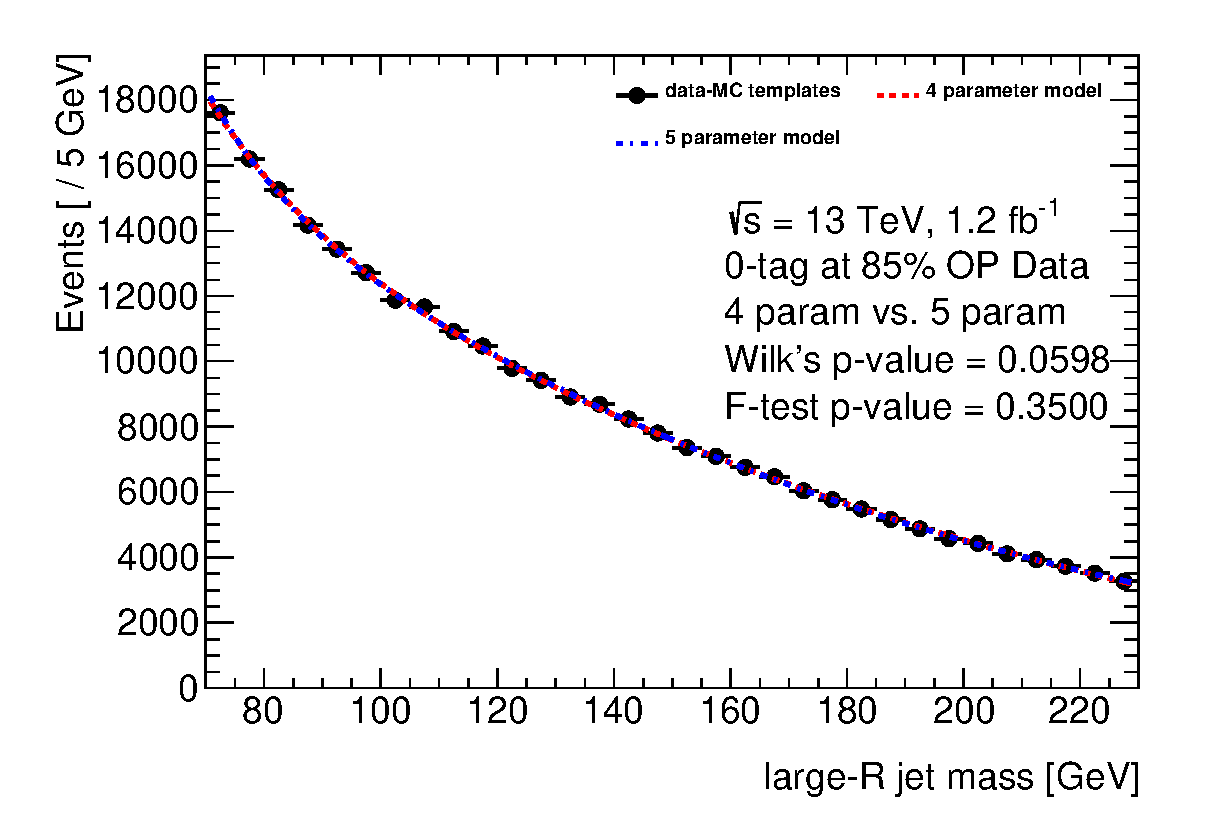
\includegraphics[width=\textwidth]{analysis/stat_test_laurent_4_v_5params_CR_data.eps}
  \caption[Comparison of the Formal Laurent fit models with 4 and 5 parameters.]{%
   Statistical test results of comparison of the Formal Laurent fit models with 4 and 5 parameters.}
  \label{fig:stat_test_laurent_4_v_5params_CR_data}
 \end{subfigure}%
 ~
 \begin{subfigure}[t]{0.333\textwidth}
  \centering
  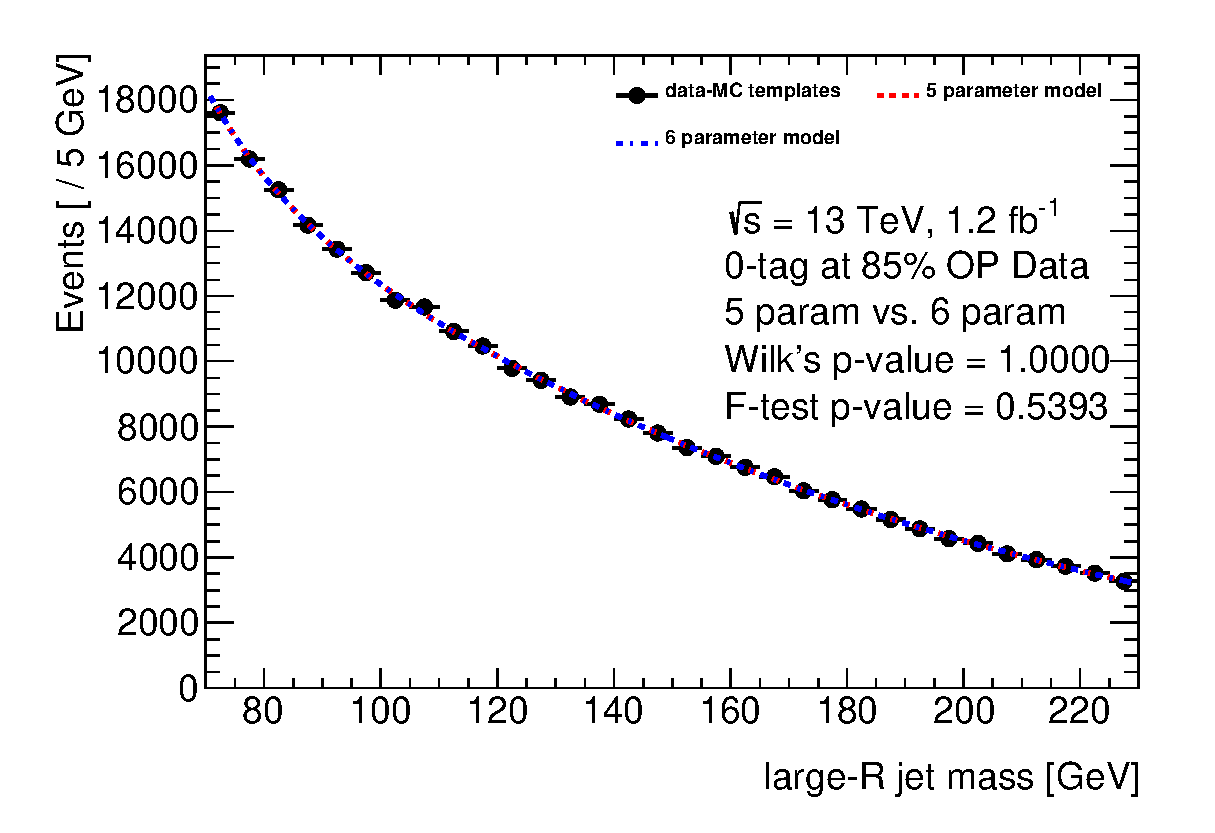
\includegraphics[width=\textwidth]{analysis/stat_test_laurent_5_v_6params_CR_data.eps}
  \caption[Comparison of the Formal Laurent fit models with 5 and 6 parameters.]{%
   Statistical test results of comparison of the Formal Laurent fit models with 5 and 6 parameters.}
  \label{fig:stat_test_laurent_5_v_6params_CR_data}
 \end{subfigure}%
 \caption[The results of the likelihood ratio test and $F$-test comparing the Formal Laurent fit models to \CRQCD{} data minus resonant Monte Carlo templates.]{%
  The results of the likelihood ratio test and $F$-test comparing the Formal Laurent fit models to \CRQCD{} data minus resonant Monte Carlo templates.}
 \label{fig:likelihood_ratio_test_laurent}
\end{figure}

\begin{table}[htbp]
 \centering
 \caption{The observed \pvalue{}s for the likelihood ratio test and $F$-test for comparing the Formal Laurent model with different number of parameters.}
 \label{table:stat_test_parameters_laurent}
 \begin{tabular}{@{}crr@{}} \toprule
  Parameters in compared models & likelihood ratio test \pvalue{} & $F$-test \pvalue{} \\ \midrule
  3 v. 4                        & $<0.0001$                       & $0.0001$           \\
  4 v. 5                        & $0.0598$                        & $0.3500$           \\
  5 v. 6                        & $1$                             & $0.5393$           \\
  \bottomrule
 \end{tabular}
\end{table}

\begin{figure}[htbp]
 \centering
 \begin{subfigure}[t]{0.48\textwidth}
  \centering
  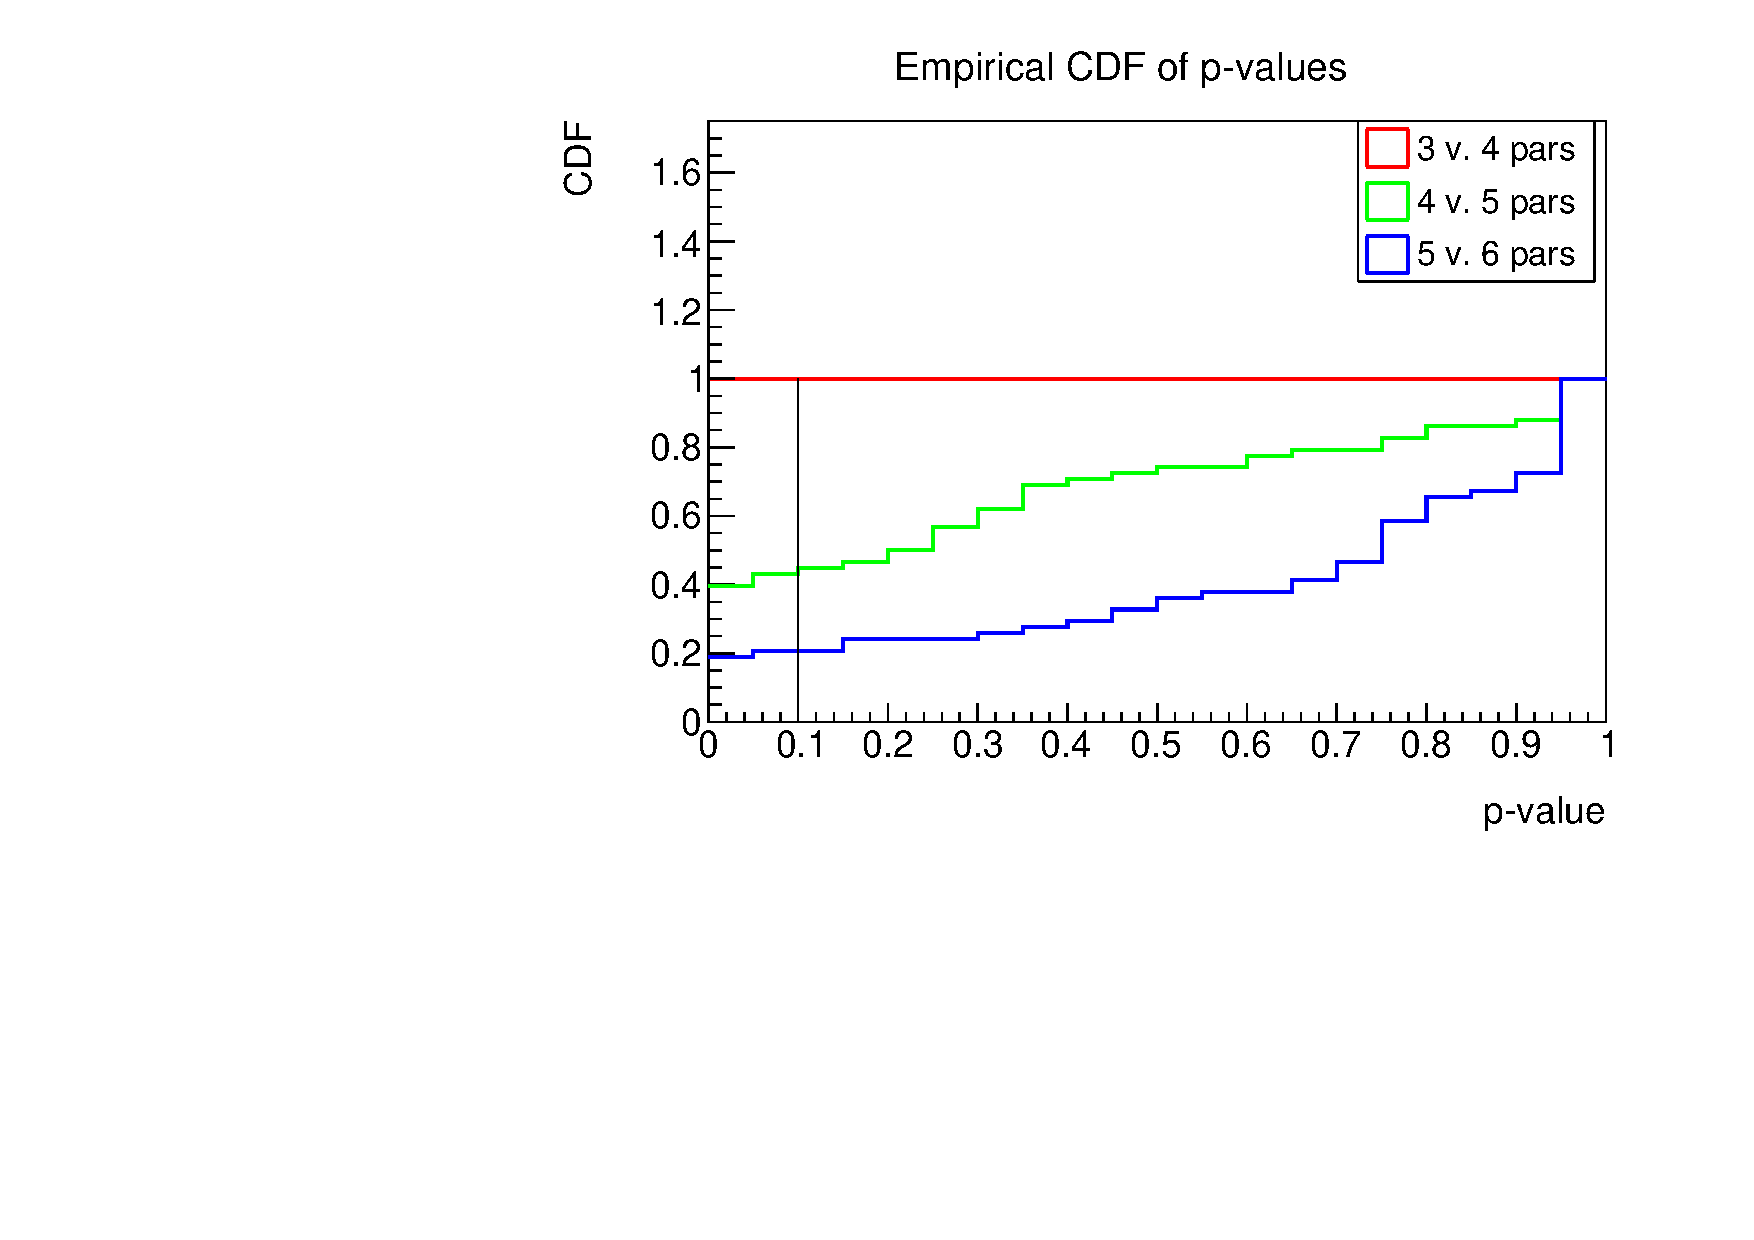
\includegraphics[width=\textwidth]{analysis/LLR_CDF_compare_Laurent.pdf}
  \caption[Empirical cumulative distribution function for the observed \pvalue{}s from the likelihood ratio test for the Formal Laurent series.]{%
   Empirical cumulative distribution function for the observed \pvalue{}s from the likelihood ratio test for the Formal Laurent series.}
  \label{fig:LLR_CDF_compare_Laurent}
 \end{subfigure}%
 \quad
 \begin{subfigure}[t]{0.48\textwidth}
  \centering
  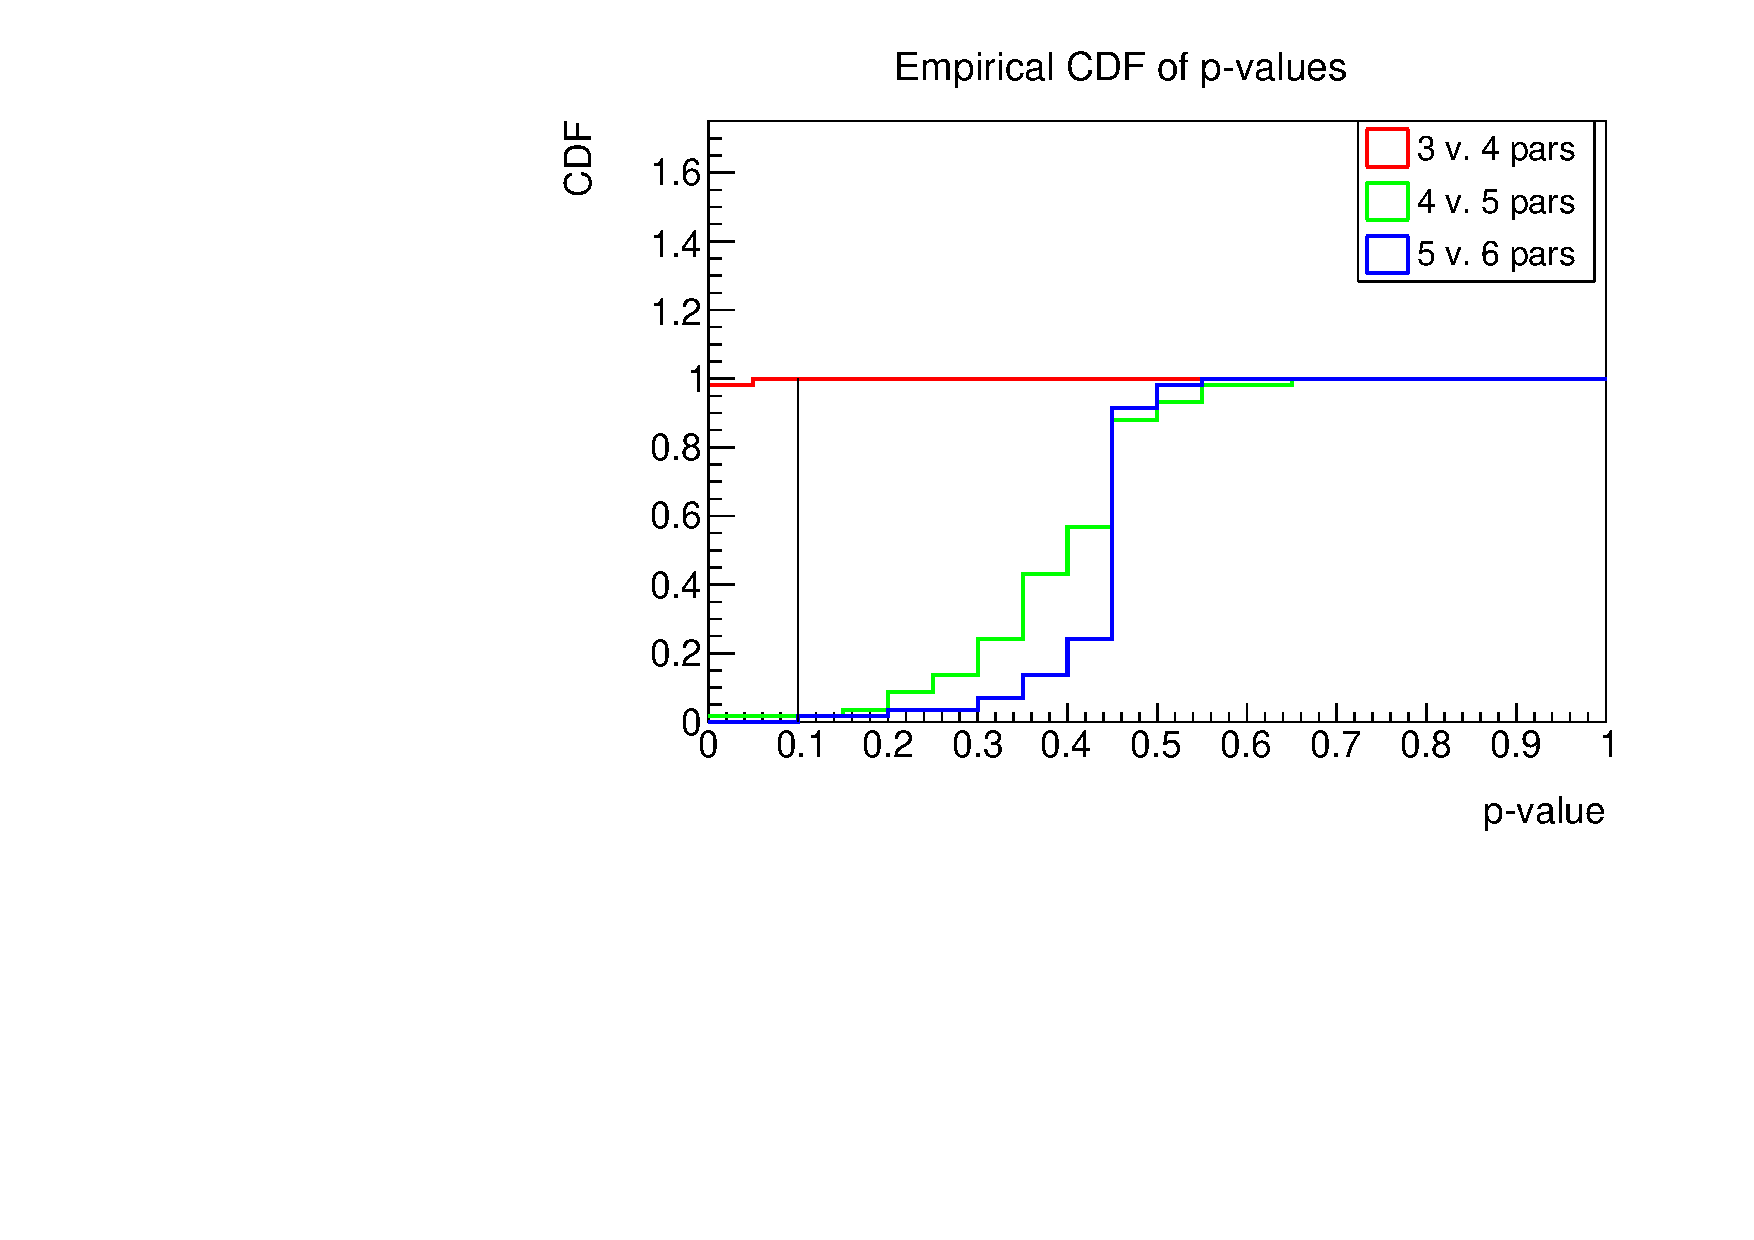
\includegraphics[width=\textwidth]{analysis/Ftest_CDF_compare_Laurent.pdf}
  \caption[Empirical cumulative distribution function for the observed \pvalue{}s from the $F$-test for the Formal Laurent series.]{%
   Empirical cumulative distribution function for the observed \pvalue{}s from the $F$-test for the Formal Laurent series.}
  \label{fig:Ftest_CDF_compare_Laurent}
 \end{subfigure}%
 \caption[Empirical cumulative distribution function for the observed \pvalue{}s for the Formal Laurent series.]{%
  Empirical cumulative distribution function for the observed \pvalue{}s for the Formal Laurent series.
  The threshold value of $\alpha=0.1$ is indicated by a vertical line.
  The likelihood ratio test favors a 5 parameter model while the $F$-test favors a 4 parameter model.}
 \label{fig:empirical_CDF_laurent}
\end{figure}

\begin{figure}[htbp]
 \centering
 \begin{subfigure}[t]{0.48\textwidth}
  \centering
  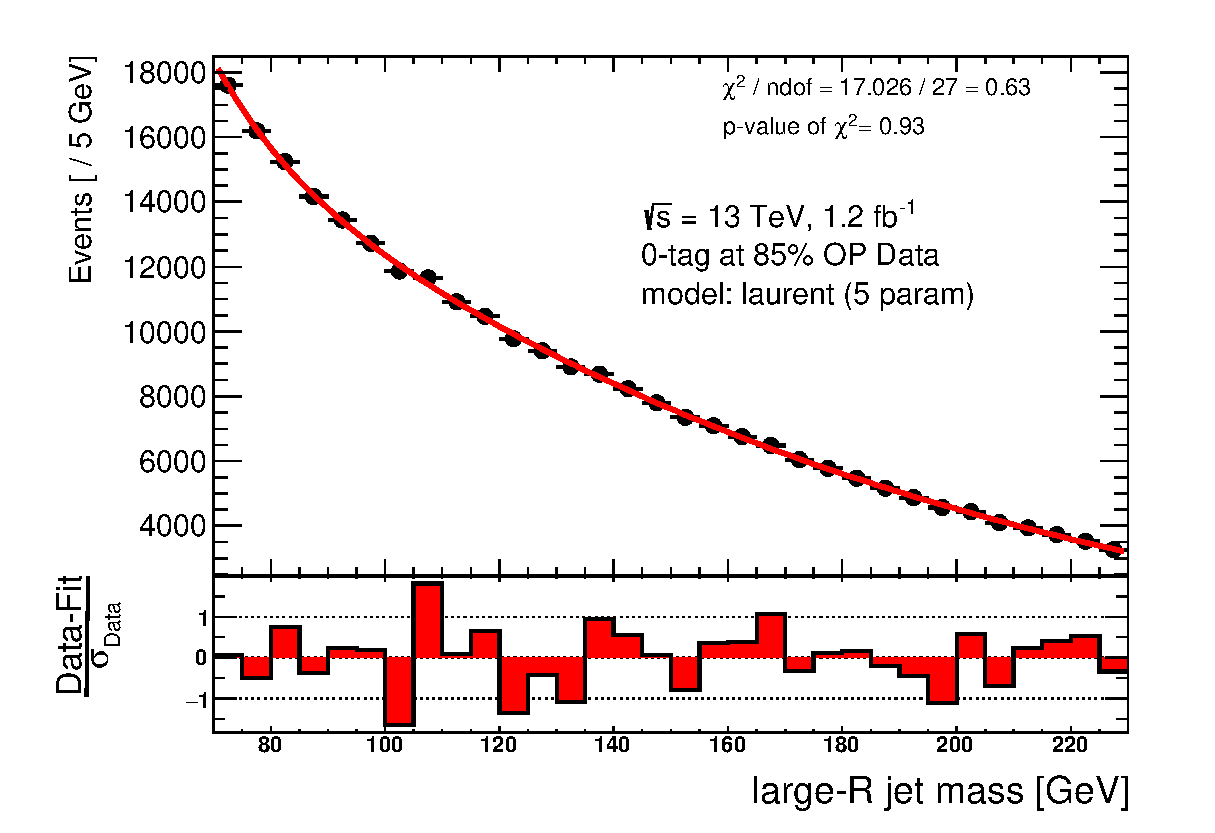
\includegraphics[width=\textwidth]{analysis/fit_5param_laurent_to_CR_data_1_2ifb.eps}
  \caption[The fit of the 5 parameter Formal Laurent model to a slice of the \CRQCD{} data.]{%
   The fit of the 5 parameter Formal Laurent model to a $1.2~\ifb$ slice of the \CRQCD{} data with the resonant Monte Carlo templates subtracted.}
  \label{fig:fit_5param_laurent_to_CR_data_1_2ifb}
 \end{subfigure}%
 \quad
 \begin{subfigure}[t]{0.48\textwidth}
  \centering
  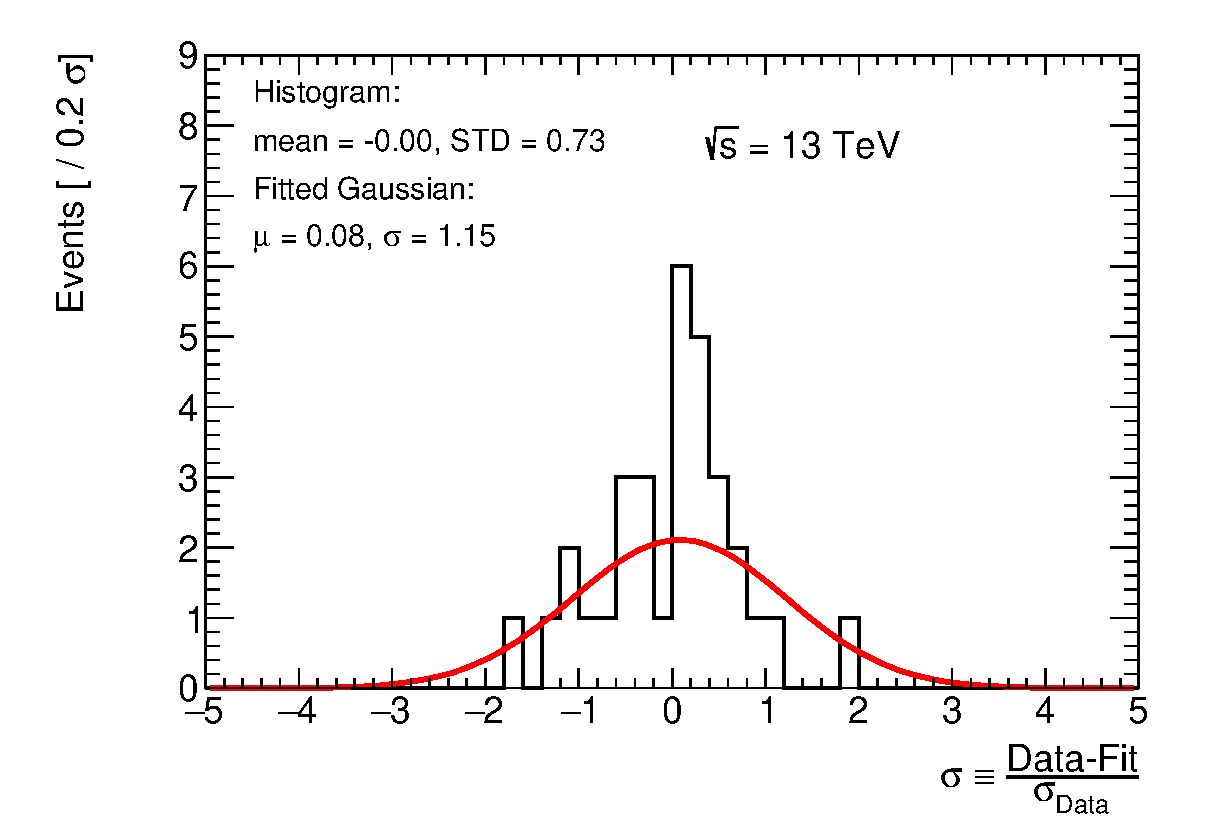
\includegraphics[width=\textwidth]{analysis/sig_dist_5param_laurent_to_CR_data_1_2ifb.eps}
  \caption[Distribution of the weighted residuals of the fit.]{%
   Distribution of the weighted residuals of the fit.}
  \label{fig:sig_dist_5param_laurent_to_CR_data_1_2ifb}
 \end{subfigure}%
 \caption[The fit and fit residuals of the 5 parameter Formal Laurent model to a slice of the \CRQCD{} data.]{%
  The fit of the 5 parameter Formal Laurent model to a $1.2~\ifb$ slice of the \CRQCD{} data with the resonant Monte Carlo templates subtracted.
  The fit exhibits both a low reduced $\chi^{2}$ value and a high \pvalue{} for the $\chi^{2}$ indicating a good fit.
  The distribution of the weighted residuals of the fit with a Normal distribution fitted to it.
  Though with low statistics at only 32 entries given the mass binning of $5~\GeV$, the residuals appear to be Normally distributed, which again indicates a good fit.}
 \label{fig:5param_QCD_model_fit_laurent}
\end{figure}

\clearpage
\section{Systematic Uncertainties}\label{sec:systematic_uncertainties}

The following section is a short discussion of sources of systematic uncertainty (``systematics'') in the analysis that could result in biases.
These uncertainties can be related to experimental calibrations or procedures and to MC modeling of signal and background processes.
These uncertainties contribute both to the uncertainties in the overall yield (``normalization'') and the differential shape of the distribution in the \largeR{} jet mass observable (``shape'') that is used in the statistical procedure for the search.

Systematic uncertainties associated with the multijet background are estimated with pseudoexperiments.
Poisson toys are sampled from the QCD component of the fit in the SR containing all components of the full model (QCD, $\Vjets$, $\ttbar$, and the exotic or Higgs boson signal components) and no nuisance parameters.
The toys are then fit with the nominal QCD parametric model (the polynomial exponential) and the alternative model (the Formal Laurent series).
These two sets of fits to the toys provide a measure of the statistical uncertainty on the multijet parameterization from the spread of the fit parameters and of the systematic uncertainty from the choice of fitting function from the difference between the two fitted shapes.

Uncertainties related to the \largeR{} jet energy and mass calibrations~\cite{JETM-2018-02} and the calibration of the \texttt{MV2c10} $b$-tagging algorithm~\cite{PERF-2016-05}, which affects different jet flavors differently, affect all of the MC templates.
The \largeR{} jet energy and mass calibration uncertainties affect both the shape and the normalization of the MC templates, so their impact on the analysis is determined by varying the jet energy and jet mass within their uncertainties and propagating those variations through the analysis.
The effect of the jet energy resolution uncertainty is tested as well, but was found to be negligible.
The effect of uncertainties on the calibration of the \texttt{MV2c10} algorithm are independent of the \largeR{} jet mass in both the signal and background simulation, and so only affect the signal normalization.

Additional shape uncertainties related to modeling generator choice are applied to the $\Vjets$ and $\ttbar$ MC templates.
To determine the systematic, the \largeR{} jet mass shapes are generated from two different MC generators and compared.
For $\Vjets$, the nominal shape, generated using \textsc{Sherpa} 2.1.1, is compared to an alternate shape, generated using \textsc{Herwrig++} 2.7.
For the $\ttbar$, the nominal \textsc{Powheg-Box} 2 shape is compared to the alternate \textsc{Sherpa} 2.2.1 shape.

The $\ttbar$ normalization in the signal region is constrained in the fit by the $k$-factor obtained from the \CRttbar{}.
The $\ttbar$ $k$-factor has an uncertainty of approximately $13\%$ of its point estimate value, and this uncertainty is used as a systematic on the $\ttbar$ normalization.

Following a methodology similar to~\cite{DAPR-2011-01}, the uncertainty on the integrated luminosity is $2.1\%$.
This systematic is then applied to all processed modeled using MC simulation.

Theoretical systematic uncertainties are added for the normalizations of the $\Vjets$ and Higgs components to the fit in the signal region.
The theory uncertainties on the $\Vjets$ result from the impact of higher order electroweak and QCD corrections to the differential cross sections for the $W+\mathrm{jets}$ and $Z+\mathrm{jets}$~\cite{Lindert:2017olm}.
The theory uncertainties for the Higgs boson production are dominated by the uncertainty on gluon-gluon fusion production, which is taken to be $30\%$, as this is consistent with the cross section uncertainty calculated with the MiNLO procedure including effects from the top-mass for Higgs boson production with $p_{T}> 400~\GeV$.
This same $30\%$ uncertainty is applied to the other Higgs production mechanisms at high $p_{T}$, which results in the total theory uncertainty on the Higgs cross section to be $30\%$.

The impact of a systematic uncertainty is defined as the difference in quadrature between the uncertainty in $\mu$ computed when all other uncertainties are considered and when they are fixed to their pre-fit values.
The total systematic uncertainty is then defined as the difference in quadrature between the total uncertainty in $\mu$ and the total statistical uncertainty~\cite{ATLAS-CONF-2018-052}.
The systematic uncertainties and their impacts on the measurement of the signal strengths are summarized in \Cref{table:systematic_uncertainties}.
It is seen that the jet mass resolution is a large systematic for all the signals.
Given that the ATLAS detector is designed for excellent energy resolution, as compared to mass resolution, this systematic will not diminish much.
However, as there are efforts to bring particle flow (``pflow'')~\cite{PERF-2015-09} into \largeR{} jets in ATLAS then future versions of this analysis might be able to improve upon this systematic given the additional use of tracking information to improve mass resolution.
The theory systematic for the Higgs is large at $30\%$; however, as noted at the start of this chapter, for some models for anomalous couplings in Higgs production the effect size at high $p_{T}$ would be greater than $30\%$~\cite{Grojean:2013nya,Dawson:2015gka}, and so this analysis could have sensitivity to such models despite the systematic's size.

\begin{table}[htpb]
 \centering
 \caption[Summary of the impact of the main systematic uncertainties on the signal strength uncertainties.]{%
  Summary of the impact $(\sqrt{\Delta \sigma^2}/\mu)$ of the main systematic uncertainties on the uncertainty, $\sigma$, on the measurement of the signal strength, $\mu$, for the $\Vjets$, Higgs boson and $\Zprime$ signals~\cite{ATLAS-CONF-2018-052}.}
 \begin{adjustbox}{max width=\textwidth}
  \begin{tabular}{@{}llrrrr@{}}
   \toprule
   Source                    & Type           & $\Vjets$ & Higgs  & $\Zprime$ $\left(100~\GeV\right)$ & $\Zprime$ $\left(175~\GeV\right)$ \\ \midrule
   Jet energy and mass scale & Norm. \& Shape & $15\%$   & $14\%$ & $23\%$                            & $18\%$                            \\
   Jet mass resolution       & Norm. \& Shape & $20\%$   & $17\%$ & $30\% $                           & $20\% $                           \\
   $V$ + jets modeling       & Shape          & $9\%$    & $4\%$  & $4\%$                             & $<1\%$                            \\
   $t\bar{t}$ modeling       & Shape          & $<1\%$   & $1\%$  & $<1\%$                            & $11\%$                            \\
   $b$-tagging $(b)$         & Normalization  & $11\%$   & $12\%$ & $11\%$                            & $15\%$                            \\
   $b$-tagging $(c)$         & Normalization  & $3\%$    & $1\%$  & $3\%$                             & $5\%$                             \\
   $b$-tagging $(l)$         & Normalization  & $4\%$    & $1\%$  & $4\%$                             & $7\%$                             \\
   $t\bar{t}$ $k$-factor     & Normalization  & $2\%$    & $3\%$  & $2\%$                             & $58\%$                            \\
   Luminosity                & Normalization  & $2\%$    & $2\%$  & $2\%$                             & $3\%$                             \\
   Alternate QCD function    & Norm. \& Shape & $4\%$    & $4\%$  & $3\%$                             & $17\%$                            \\
   $W$/$Z$ and QCD (Theory)  & Normalization  & $14\%$   &        &                                   &                                   \\
   Higgs (Theory)            & Normalization  &          & $30\%$ &                                   &                                   \\
   \bottomrule
  \end{tabular}
 \end{adjustbox}
 \label{table:systematic_uncertainties}
\end{table}
